% ==========================================
% LatexRefinement Step Output: step4-05-05-25-tuesday-all-offset-final.tex
% Model: gemini-3.5-flash
% Temperature: 0.36
% TopP: 0.95
% TopK: 40
% MaxOutputTokens: 65535
% ThinkingBudget: 32768
% ThinkingLevel: HIGH
% Prompt Tokens: 38'456
% Candidates Tokens: 27'090 (inkl. Thinking Tokens)
% Cached Tokens: 0
% Processed on: 2026-07-10 13:49:53
% ==========================================

\lecturechapter[11]{Dienstag}{5. Mai}{5. Mai 2026}{Graphentheorie}

\begin{nice-box}[Syllabus / Agenda]
In dieser Vorlesung beschäftigen wir uns mit den folgenden zentralen Themen der Graphentheorie:
\begin{itemize}
    \item \textbf{Das Handschlaglemma:} Formulierung, Beweis und alltägliche Interpretation.
    \item \textbf{Euler-Linien und Euler-Graphen:} Der Satz von Euler, das Königsberger Brückenproblem und das Dominoproblem als praktische Anwendung.
    \item \textbf{Hamilton-Kreise und Hamilton-Graphen:} Definition, Beispiele (platonische Körper, Hyperwürfel) und die Konstruktion von Gray-Codes.
    \item \textbf{Bipartite Graphen:} Definition, Zwei-Färbbarkeit und Nachbarschaften.
    \item \textbf{Der Heiratssatz von Hall:} Formulierung, Interpretation und ein vollständiger Induktionsbeweis.
\end{itemize}
\end{nice-box}

\section{Das Handschlaglemma}

\begin{spoken-clean}[00:00:00 - 00:01:58]
Hallo zusammen, wir fangen an. Herzlich willkommen zur elften Woche. Wir sind noch mittendrin in der Graphentheorie --- also ein ganz kleiner Einblick in ein bisschen, um was es in der Graphentheorie, Teilen der Graphentheorie geht.

Letzte Woche haben wir noch kurz mit dem einen Lemma aufgehört. Ich wollte das noch kurz umformulieren: Dieses Lemma heißt auch das Handschlaglemma. \inlinemetanote{schreibt an die Tafel} Das Schöne an der Graphentheorie ist, man kann sie oft so in alltägliche Situationen umformen --- oder viele Sachen sind vielleicht auch Probleme aus dem realen Leben ---, und dann kann man, wenn man sieht, dass das einfach ein Graphenproblem ist, das mit irgendeinem graphentheoretischen Lemma lösen.

Das Handschlaglemma sagt: Auf einer Party mit $n$ Gästen ist die Anzahl der Gäste, die einer ungeraden Anzahl von Gästen die Hand geben, gerade. Okay, und das war im Prinzip genau das, was wir am Ende der letzten Stunde bewiesen haben.
\end{spoken-clean}

\begin{math-stroke}
\begin{lemma}[Handschlaglemma]\label[lemma]{lem:handschlaglemma}
Auf einer Party mit $n$ Gästen ist die Anzahl der Gäste, die einer ungeraden Anzahl von Gästen die Hand geben, gerade.
\end{lemma}
\end{math-stroke}

\begin{proof}[Beweis des Handschlaglemmas]
\begin{spoken-clean}[00:01:58 - 00:03:38]
Der Beweis ist: \inlinemetanote{schreibt an die Tafel} Wir betrachten einfach den Graphen $G = (V, E)$, wobei $V$ genau die Gäste sind, und $E$ --- da es ein ungerichteter Graph ist --- einfach die Paare von Gästen sind, die sich die Hand geben. Und wir haben gesehen, dass die Anzahl der $x \in V$, sodass der Grad von $x$ ungerade ist, immer gerade ist.

Vielleicht, okay, wir gehen natürlich davon aus, dass sich die Leute nicht selbst die Hand schütteln. Das geht nicht. Oder wenn man sich selbst die Hand schüttelt, dann zählt das wie zweimal die Hand schütteln, weil man sich ja selbst quasi die Hand geschüttelt hat. Also machen wir nicht. Also einfach nur, um zu sagen, dass das der Fall ist --- gut, sich eine konkrete Situation von gewissen Resultaten vorzustellen.
\end{spoken-clean}

\begin{math-stroke}
Betrachte den ungerichteten Graphen $G = (V, E)$, wobei:
\begin{itemize}
    \item \textbf{V:} $V := \{\text{Gäste}\}$
    \item \textbf{E:} $E := \{\{x, y\} \mid x \text{ und } y \text{ geben sich die Hand}\}$
\end{itemize}
Aus dem allgemeinen Handschlaglemma für Graphen wissen wir, dass die Summe der Grade aller Knoten stets gerade ist:
\[
\sum_{v \in V} \deg(v) = 2|E|
\]
Daraus folgt unmittelbar, dass die Anzahl der Knoten mit ungeradem Grad gerade sein muss:
\[
\left| \bigl\{ z \in V \;\big|\; \deg(z) \text{ ist ungerade} \bigr\} \right| \equiv 0 \pmod 2
\]
\end{math-stroke}
\end{proof}

\section{Euler-Linien und Euler-Graphen}

\begin{spoken-clean}[00:03:38 - 00:05:40]
Und das Letzte, wofür wir letzte Woche leider keine Zeit mehr hatten, war noch diese Sache mit den Euler-Linien. Das ist die folgende Definition: Eine Euler-Linie eines Graphen $G$ ist ein geschlossener Kantenzug, der sämtliche Kanten von $G$ enthält. \inlinemetanote{schreibt an die Tafel}

Okay, also wir hatten Kantenzüge nur für Graphen mit nur einer Relation definiert, aber man kann das ähnlich auch für Graphen mit Mehrfachkanten definieren --- haben wir aber nicht gemacht, das wäre einmal hier. Und es ist wirklich ein Kantenzug, das heißt, jede Kante kommt höchstens einmal vor im Kantenzug. Es dürfen aber dieselben Knoten mehrmals verwendet werden.

Und genau, wenn man einen geschlossenen Kantenzug hat, der alle Kanten von $G$ enthält, dann ist das eine eulersche Linie --- ich schreibe lieber Euler-Linie ---, also ganz gemäß dem Königsberger Brückenproblem. Und ein Graph heißt Euler-Graph, wenn er eine Euler-Linie enthält. \inlinemetanote{schreibt an die Tafel}
\end{spoken-clean}

\begin{math-stroke}
\begin{definition}[Euler-Linie und Euler-Graph]\label[definition]{def:euler-linie}
Sei $G = (V, E)$ ein ungerichteter Graph.
\begin{itemize}
    \item Eine \newterm{Euler-Linie} von $G$ ist ein geschlossener Kantenzug, der jede Kante von $G$ genau einmal enthält.
    \item Ein Graph $G$ heißt \newterm{Euler-Graph}, falls er eine Euler-Linie besitzt.
\end{itemize}
\end{definition}

\begin{explanation-of-steps}
Ein Kantenzug ist eine Folge von Knoten und Kanten, bei der sich Kanten nicht wiederholen dürfen. Knoten dürfen jedoch beliebig oft besucht werden. Ein geschlossener Kantenzug beginnt und endet am selben Knoten.
\end{explanation-of-steps}
\end{math-stroke}

\begin{ai-global-state-checkpoint-invisible-content}
% timestamp: 00:05:40
% topic: Einführung Euler-Linien und Euler-Graphen
% board_state: lem:handschlaglemma, def:euler-linie
% next_goal: Formulierung der Proposition 9.3 (Satz von Euler)
% open_loops: none
\end{ai-global-state-checkpoint-invisible-content}

\begin{spoken-clean}[00:05:40 - 00:06:45]
Okay. Also der Graph der Königsberger Brücken wäre also ein Beispiel für einen Graphen, der kein Euler-Graph ist, wohingegen das Haus vom Nikolaus ein Graph ist, der ein Euler-Graph ist, wie wir letztes Mal kurz am Anfang als Motivation diskutiert haben. Und das können wir hier noch in dieser Proposition abschließen --- das ist die Proposition \textbf{9.3}.
\end{spoken-clean}

\begin{didactic-insight}[Das Königsberger Brückenproblem]
Das historische Königsberger Brückenproblem (gelöst von Leonhard Euler im Jahr 1736) gilt als die Geburtsstunde der Graphentheorie. Die Frage war, ob man einen Spaziergang durch die Stadt Königsberg so planen kann, dass man jede der sieben Brücken genau einmal überquert und am Ende wieder am Ausgangspunkt ankommt. Euler abstrahierte die Stadtteile als Knoten und die Brücken als Kanten und zeigte, dass dies unmöglich ist, da nicht alle Knoten einen geraden Grad besitzen.
\end{didactic-insight}

\subsection{Zusammenhang und der Satz von Euler}

\begin{spoken-clean}[00:06:45 - 00:08:55]
Die sagt, dass ein endlicher, ungerichteter, zusammenhängender Graph... zusammenhängend haben wir, glaube ich, nicht definiert. Das heißt einfach das, was man denkt: Wenn man je zwei Knoten nimmt, dann existiert ein Kantenzug zwischen diesen Knoten. Man kann also je zwei Knoten miteinander verbinden --- das ist die Definition, das heißt, es existiert ein Kantenzug zwischen je zwei Knoten. \inlinemetanote{schreibt an die Tafel}

Also ein endlicher, ungerichteter, zusammenhängender Graph $G$ ist genau dann ein Euler-Graph, wenn jeder Knoten von $G$ geraden Grad hat. \inlinemetanote{schreibt an die Tafel}
\end{spoken-clean}

\begin{math-stroke}
\begin{definition}[Zusammenhängender Graph]\label[definition]{def:zusammenhaengend}
Ein Graph $G = (V, E)$ heißt \newterm{zusammenhängend}, wenn zu je zwei Knoten $u, v \in V$ ein Kantenzug existiert, der $u$ und $v$ verbindet.
\end{definition}

\begin{proposition}[Satz von Euler]\label[proposition]{prop:satz-von-euler}
Ein endlicher, ungerichteter, zusammenhängender Graph $G$ ist genau dann ein Euler-Graph, wenn jeder Knoten von $G$ einen geraden Grad besitzt:
\[
\forall v \in V \colon \deg(v) \equiv 0 \pmod 2
\]
\end{proposition}
\end{math-stroke}

\begin{proof}[Beweis des Satzes von Euler]
\begin{spoken-clean}[00:08:55 - 00:11:15]
Das ist der Satz von Euler, mit dem er gezeigt hat, dass eben das Königsberger Brückenproblem keine Lösung hat, weil man dort halt eben viele Knoten hat, die ungeraden Grad haben. Okay? Und die andere Sache ist: Es zeigt nicht nur... okay, Euler hat gesehen, das ist eine notwendige Bedingung, also wenn es ein Euler-Graph ist, dann muss diese Bedingung erfüllt sein. Aber das ist eben auch eine hinreichende Bedingung: Wenn alle Knoten einen geraden Grad haben, dann gibt es eine Euler-Linie.

Okay. Ja, der Beweis ist im Wesentlichen einfach das Argument von Euler. Falls $G$ eine Euler-Linie hat, so ist jeder Knoten von $G$ von geradem Grad, weil er so oft Anfangs- wie Endpunkt dieser Linie ist. \inlinemetanote{schreibt an die Tafel} Und genau, daraus folgt, dass jeder Knoten einen geraden Grad hat.
\end{spoken-clean}

\begin{math-stroke}
\textbf{Hinrichtung (\texorpdfstring{\textbf{(a)} $\implies$ \textbf{(b)}}{a -> b}):}
Sei $G$ ein Euler-Graph mit einer Euler-Linie $L$. Da $L$ ein geschlossener Kantenzug ist, der jede Kante von $G$ genau einmal enthält, können wir die Kanten entlanggehen. 

Bei jedem Durchgang durch einen Knoten $v \in V$ betreten wir den Knoten über eine Kante und verlassen ihn über eine andere Kante. Jedes Mal, wenn die Linie $L$ den Knoten $v$ passiert, werden somit genau zwei Kanten verbraucht, die an $v$ angrenzen. 

Da jede Kante von $G$ in $L$ genau einmal vorkommt, muss der Grad jedes Knotens $v$ gerade sein, da er sich als das Doppelte der Anzahl der Durchgänge durch $v$ darstellt (wobei der Start- und Endknoten der Linie beim ersten Verlassen und letzten Betreten ebenfalls genau zwei Kanten beisteuert). Somit gilt:
\[
\forall v \in V \colon \deg(v) \equiv 0 \pmod 2
\]
\end{math-stroke}

\begin{spoken-clean}[00:11:15 - 00:13:38]
Und für die Umkehrung beziehungsweise die Rückrichtung konstruieren wir so eine Euler-Linie, wenn wir wissen, dass das der Fall ist. Zuerst einmal, okay, er ist zusammenhängend; und wenn der Graph zusammenhängend ist, dann heißt das insbesondere, dass es keine Knoten gibt von Ordnung Null (d.\,h.\ isolierte Knoten). Wenn ein Knoten von Ordnung Null wäre, dann könnte man ihn mit niemandem verbinden. Das heißt, jeder Knoten hat mindestens Grad \textbf{2}. \inlinemetanote{schreibt an die Tafel}

\inlinemetanote{(Zunächst einmal ist der Graph zusammenhängend. Das bedeutet insbesondere, dass es keine isolierten Knoten vom Grad $0$ gibt --- denn einen solchen Knoten könnte man ja mit keinem anderen verbinden. Da alle Grade gerade und größer als $0$ sein müssen, hat jeder Knoten mindestens den Grad $2$.)}

Und was wir jetzt tun: Wir nehmen einen Knoten $x_0$. Wir starten jetzt an einem Knoten $x_0$, wir beginnen jetzt bei $x_0$, und jetzt laufen wir einfach los zu irgendeinem anderen Knoten $x_1$, $x_2$ und so weiter. Und zwar starten wir im Knoten $x_0$, und dann gehen wir vom Knoten $x_i$ weiter zum Knoten $x_{i+1}$ --- und das immer auf einer Kante, die wir noch nicht besucht haben, also auf einer, sagen wir mal, unbesuchten Kante. \inlinemetanote{schreibt an die Tafel}
\end{spoken-clean}


\begin{ai-global-state-checkpoint-invisible-content}
% timestamp: 00:12:00
% topic: Beweis des Satzes von Euler (Rückrichtung)
% board_state: prop:satz-von-euler, proof:euler-forward
% next_goal: Konstruktion des geschlossenen Kantenzugs K_0
% open_loops: none
\end{ai-global-state-checkpoint-invisible-content}

\begin{math-stroke}
\textbf{Rückrichtung (\texorpdfstring{\textbf{(b)} $\implies$ \textbf{(a)}}{b -> a}) --- Teil 1:}
Wir nehmen an, dass jeder Knoten von $G$ einen geraden Grad besitzt. Da $G$ zusammenhängend ist und wir triviale isolierte Knoten ausschließen, gilt:
\[
\forall v \in V \colon \deg(v) \ge 2
\]
Wir starten die Konstruktion an einem beliebigen Knoten $x_0 \in V$. Wir bilden einen Kantenzug, indem wir von einem Knoten $x_i$ zu einem Nachbarknoten $x_{i+1}$ über eine noch unbesuchte Kante gehen.
\end{math-stroke}

\begin{spoken-clean}[00:13:38 - 00:15:10]
Und das können wir immer, weil wenn wir auf einer unbesuchten Kante in einen Knoten reingehen, dann gibt es auch noch eine unbesuchte Kante, die wieder rausgeht, weil sonst hätte der entsprechende Knoten ja eine ungerade Ordnung (d.\,h.\ einen ungeraden Grad).

Okay, und jetzt irgendwann kommen wir... also $G$ ist ein endlicher Graphen. Das heißt, wir kommen irgendwann zurück zu $x_0$. \inlinemetanote{schreibt an die Tafel} Das heißt, es existiert ein geschlossener Kantenzug --- $K_0$ nennen wir ihn --- beginnend in $x_0$. Okay, und falls dieser $K_0$ jetzt bereits alle Kanten enthält, ist gut, dann sind wir fertig.

Okay, wenn es jetzt aber noch Kanten gibt, die nicht in $K_0$ enthalten sind, dann muss einer der Knoten, die auf $K_0$ liegen, an eine solche (unbesuchte) Kante angrenzen, weil der Graph ja zusammenhängend ist. Es kann also nicht sein, dass alle unbesuchten Kanten nicht an die Knoten in $K_0$ angrenzen.
\end{spoken-clean}

\begin{math-stroke}
\textbf{Rückrichtung (\texorpdfstring{\textbf{(b)} $\implies$ \textbf{(a)}}{b -> a}) --- Teil 2:}
Da jeder Knoten geraden Grad hat, können wir, wann immer wir einen Knoten $v \neq x_0$ betreten, diesen auch wieder über eine unbesuchte Kante verlassen. Da der Graph $G$ endlich ist, müssen uns irgendwann die unbesuchten Kanten ausgehen. Dies kann nur am Startknoten $x_0$ geschehen. 

Somit erhalten wir einen ersten geschlossenen Kantenzug $K_0$, der in $x_0$ startet und endet.
\[
\text{Falls } E(K_0) = E(G), \text{ dann ist } K_0 \text{ eine Euler-Linie und wir sind fertig.}
\]
Falls noch unbesuchte Kanten existieren, so muss wegen des Zusammenhangs von $G$ mindestens eine dieser Kanten an einen Knoten $x_n \in V(K_0)$ angrenzen.
\end{math-stroke}

\begin{spoken-clean}[00:15:10 - 00:17:28]
Es gibt also auf $K_0$ einen Knoten --- nennen wir ihn $x_n$ ---, von dem natürlich eine gerade Anzahl von Kanten ausgeht, die nicht auf $K_0$ liegen. Wir haben hier also unseren geschlossenen Kantenzug $K_0$ von $x_0$ nach $x_0$, irgendwo liegt $x_n$, und von dort gehen noch unbesuchte Kanten aus --- und zwar eine gerade Anzahl.

Jetzt machen wir an dieser Stelle genau dasselbe: Wir starten in $x_n$ und laufen entlang neuer Kanten, bis wir wieder zu $x_n$ zurückkehren. Wir erhalten so einen weiteren geschlossenen Kantenzug $K_1$. Nun können wir diese beiden Kantenzüge ganz einfach zusammenhängen: Wir laufen zuerst auf $K_0$ bis $x_n$, durchlaufen dann den gesamten Kantenzug $K_1$, und setzen danach den Weg auf $K_0$ fort. So erhalten wir einen neuen, größeren geschlossenen Kantenzug.

Dieses Verfahren wiederholen wir nun so lange, bis wir eine Euler-Linie haben. Das funktioniert deshalb, weil wir in jedem Schritt nur eine gerade Anzahl von Kanten entfernen, sodass die verbleibenden unbesuchten Kanten in jedem Knoten weiterhin einen geraden Grad aufweisen.
\end{spoken-clean}

\begin{math-stroke}
\textbf{Rückrichtung (\texorpdfstring{\textbf{(b)} $\implies$ \textbf{(a)}}{b -> a}) --- Teil 3:}
Wir betrachten den Teilgraphen $G' = (V, E \setminus E(K_0))$. In $G'$ hat jeder Knoten weiterhin einen geraden Grad. 

Sei $x_n \in V(K_0)$ ein Knoten, der eine unbesuchte Kante in $G'$ besitzt. Wir starten in $x_n$ und konstruieren analog zu $K_0$ einen geschlossenen Kantenzug $K_1$ in $G'$, der in $x_n$ beginnt und endet.

Wir können nun $K_0$ und $K_1$ zu einem einzigen, größeren geschlossenen Kantenzug verbinden, indem wir $K_0$ bis zum Knoten $x_n$ durchlaufen, dann den gesamten Kantenzug $K_1$ abschreiten, und anschließend den Rest von $K_0$ bis $x_0$ vollenden.

\begin{center}
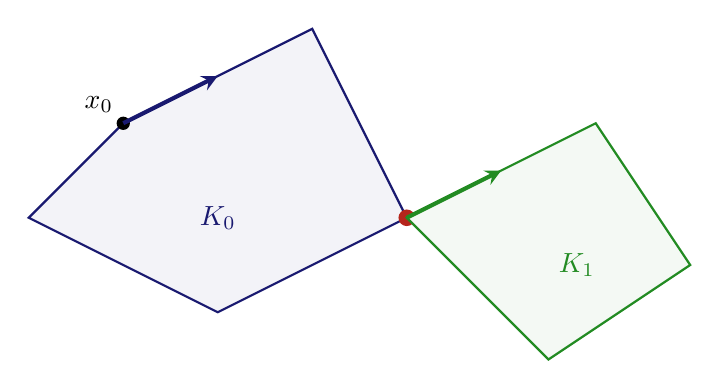
\begin{tikzpicture}[scale=1.2, >=stealth, thick]
  % \begin{ai-tikz-planner-invisible-content}
  % 1. Background: Kantenzug K_0 als lila Fünfeck.
  % 2. Midground: Kantenzug K_1 als grünes Viereck, das K_0 im Knoten x_n schneidet.
  % 3. Foreground: Pfeile, die den Durchlaufweg andeuten.
  % \end{ai-tikz-planner-invisible-content}
  
  % K_0 (lila)
  \draw[MidnightBlue, fill=MidnightBlue!5] (0,0) -- (2,1) -- (3,-1) -- (1,-2) -- (-1,-1) -- cycle;
  \node[MidnightBlue] at (1,-1) {$K_0$};
  \fill (0,0) circle (2pt) node[above left] {$x_0$};
  
  % Schnittknoten x_n
  \coordinate (Xn) at (3,-1);
  \fill[BrickRed] (Xn) circle (2.5pt) node[right=3pt] {$x_n$};
  
  % K_1 (grün)
  \draw[ForestGreen, fill=ForestGreen!5] (3,-1) -- (5,0) -- (6,-1.5) -- (4.5,-2.5) -- cycle;
  \node[ForestGreen] at (4.8,-1.5) {$K_1$};
  
  % Durchlaufpfeile
  \draw[->, MidnightBlue, line width=1.5pt] (0,0) -- (1,0.5);
  \draw[->, ForestGreen, line width=1.5pt] (3,-1) -- (4, -0.5);
\end{tikzpicture}
\end{center}

Da der Graph $G$ endlich ist, führt die wiederholte Anwendung dieses Verfahrens nach endlich vielen Schritten zu einem geschlossenen Kantenzug, der alle Kanten von $G$ enthält. Dies beweist, dass $G$ ein Euler-Graph ist.
\end{math-stroke}
\end{proof}

\begin{ai-global-state-checkpoint-invisible-content}
% timestamp: 00:18:00
% topic: Abschluss Satz von Euler, Einführung offene Euler-Linien
% board_state: prop:satz-von-euler, proof:euler-backward-complete
% next_goal: Formulierung des Korollars für offene Euler-Linien
% open_loops: none
\end{ai-global-state-checkpoint-invisible-content}

\subsection{Offene Euler-Linien}
% New subsection: Offene Euler-Linien

\begin{spoken-clean}[00:17:28 - 00:18:56]
Gut, soweit klar? Ich denke, die Idee des Beweises ist klar. Man kann das natürlich mehr oder weniger detailliert aufschreiben --- da gibt es verschiedene Möglichkeiten. Das hier ist eine Variante, vielleicht etwas kompakter, aber die Grundidee ist das Entscheidende.

Es gibt auch noch andere Versionen dieses Satzes, die wir hier nicht im Detail besprechen, die Sie aber im Skript nachlesen können. Bisher haben wir über geschlossene Euler-Linien gesprochen, aber man kann auch eine offene Euler-Linie definieren. Das ist ein Kantenzug, der zwar alle Kanten des Graphen $G$ enthält, aber nicht am selben Knoten beginnt, an dem er endet.

Auch hier lässt sich zeigen: Ein endlicher, ungerichteter Graph $G$ besitzt genau dann eine offene Euler-Linie, wenn er zusammenhängend ist und genau zwei Knoten mit ungeradem Grad existieren. In diesem Fall beginnen wir den Kantenzug an dem einen Knoten mit ungeradem Grad und beenden ihn an dem anderen.
\end{spoken-clean}

\begin{math-stroke}[Offene Euler-Linien]
\begin{definition}[Offene Euler-Linie]\label[definition]{def:offene-euler-linie}
Eine \newterm{offene Euler-Linie} in einem ungerichteten Graphen $G = (V, E)$ ist ein (nicht geschlossener) Kantenzug, der jede Kante von $G$ genau einmal enthält.
\end{definition}

\begin{corollary}[Existenz einer offenen Euler-Linie]\label[corollary]{cor:offene-euler-linie}
Ein endlicher, ungerichteter Graph $G$ besitzt genau dann eine offene Euler-Linie, wenn $G$ zusammenhängend ist (bis auf isolierte Knoten) und genau zwei Knoten $u, v \in V$ ungeraden Grad besitzen. In diesem Fall beginnt die offene Euler-Linie in $u$ und endet in $v$ (oder umgekehrt).
\end{corollary}
\end{math-stroke}

\begin{spoken-clean}[00:18:56 - 00:20:20]
Ähnliche Resultate gibt es auch für gerichtete Graphen --- das ist die Proposition 9.16 im Skript, die Sie dort gerne nachlesen können.
\end{spoken-clean}

\begin{math-stroke}[Weitere Versionen des Satzes]
\begin{remark}[Gerichtete Euler-Graphen]\label[remark]{rem:gerichtete-euler-graphen}
Für gerichtete Graphen gilt ein analoges Resultat (siehe Proposition 9.16 im Skript): Ein gerichteter, stark zusammenhängender Graph besitzt genau dann einen geschlossenen Euler-Zug, wenn für jeden Knoten der Eingangsgrad gleich dem Ausgangsgrad ist:
\[
\forall v \in V \colon d_{\text{in}}(v) = d_{\text{out}}(v)
\]
\end{remark}
\end{math-stroke}

\section{Das Dominoproblem}

\subsection{Das Dominoproblem und seine mathematische Modellierung}

\begin{spoken-clean}[00:20:20 - 00:22:30]
Kommen wir nun zu einer netten kleinen Anwendung dieses Satzes auf ein Problem aus dem Alltag: dem Dominoproblem. Ich weiß nicht, ob Sie heute noch oft Domino spielen, aber betrachten wir folgendes Szenario: Wir haben ein Dominospiel mit den Augenzahlen $0$ bis $16$ und den entsprechenden Dominosteinen.

Ein Dominostein sieht bekanntlich so aus: Er hat zwei Hälften mit jeweils einer Zahl, sagen wir $m$ und $n$, die beide zwischen $0$ und $16$ liegen. Für jedes ungeordnete Paar $\{m, n\}$ gibt es genau einen Stein --- es wird also nicht zwischen $\{m, n\}$ und $\{m, n\}$ unterschieden. Die Frage ist nun: Wie viele Steine hat ein solches Dominospiel insgesamt?
\end{spoken-clean}

\begin{math-stroke}[Mathematische Formulierung des Dominoproblems]
Wir betrachten ein Dominospiel mit den Augenzahlen $\{0, 1, \dots, 16\}$.
Ein Dominostein wird repräsentiert durch ein ungeordnetes Paar $\{m, n\}$ mit $m, n \in \{0, \dots, 16\}$. Für jedes Paar existiert genau ein Stein (inklusive der Doubletten $\{m, m\}$).
\end{math-stroke}

\begin{spoken-clean}[00:22:30 - 00:23:51]
Wie viele Möglichkeiten gibt es, zwei Zahlen aus $17$ auszuwählen? Dazu kommen noch die Doubletten, bei denen man zweimal dieselbe Zahl hat, also $0$-$0$, $1$-$1$ und so weiter. Das heißt, wir müssen noch $17$ weitere Steine dazuzählen.
\end{spoken-clean}

\begin{ai-global-state-checkpoint-invisible-content}
% timestamp: 00:24:00
% topic: Das Dominoproblem (Kombinatorik und Fragestellung)
% board_state: def:general-domino, eq:domino-count
% next_goal: Modellierung des Dominoproblems als Graph
% open_loops: none
\end{ai-global-state-checkpoint-invisible-content}

\begin{math-stroke}[Berechnung der Anzahl der Dominosteine]
Die Anzahl der Steine berechnet sich kombinatorisch aus den Paaren unterschiedlicher Zahlen plus den Doubletten (Steine mit zwei gleichen Zahlen):
\[
\text{Anzahl Steine} = \binom{17}{2} + 17 = \frac{17 \cdot 16}{2} + 17 = 136 + 17 = 153
\]
Es gibt somit insgesamt $153$ Dominosteine in diesem Spiel.
\end{math-stroke}

\begin{spoken-clean}[00:23:51 - 00:25:23]
Und die Frage ist --- das Dominoproblem fragt nun ---: Können wir alle Steine zu einer unverzweigten, geschlossenen Kette aneinanderreihen? \inlinemetanote{schreibt an die Tafel}

Okay, also gibt es das so, dass man hier irgendwie eine $1$ und eine $2$ hat, und dann hat man beim nächsten eine $2$ und eine $3$, und so weiter, bis man dann irgendwann wieder zurückkommt zu einer $1$ und hier ein $k$ oder so? \inlinemetanote{zeichnet eine Kette an die Tafel} \inlinemetanote{[Können wir die Steine also so anordnen, dass wir mit einem Stein $\{n_1, n_2\}$ beginnen, daran den Stein $\{n_2, n_3\}$ legen, und so weiter, bis wir am Ende wieder beim Ausgangswert $n_1$ ankommen?]}
\end{spoken-clean}

\begin{math-stroke}[Die Fragestellung]
\textbf{Frage:} Können wir alle $153$ Dominosteine so aneinanderreihen, dass sie eine einzige, geschlossene, unverzweigte Kette bilden?
\begin{center}
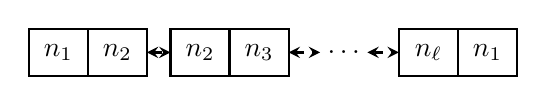
\begin{tikzpicture}[scale=1.0, >=stealth, thick]
  % \begin{ai-tikz-planner-invisible-content}
  % 1. Background: Eine Kette von Dominosteinen als Rechtecke.
  % 2. Midground: Zahlen auf den Steinen.
  % 3. Foreground: Verbindungslinien.
  % \end{ai-tikz-planner-invisible-content}
  \draw (0,0) rectangle (1.5,0.6);
  \draw (0.75,0) -- (0.75,0.6);
  \node at (0.375,0.3) {$n_1$};
  \node at (1.125,0.3) {$n_2$};
  
  \draw (1.8,0) rectangle (3.3,0.6);
  \draw (2.55,0) -- (2.55,0.6);
  \node at (2.175,0.3) {$n_2$};
  \node at (2.925,0.3) {$n_3$};
  
  \node at (4.0,0.3) {$\dots$};
  
  \draw (4.7,0) rectangle (6.2,0.6);
  \draw (5.45,0) -- (5.45,0.6);
  \node at (5.075,0.3) {$n_{\ell}$};
  \node at (5.825,0.3) {$n_1$};
  
  \draw[dashed, <->] (1.5,0.3) -- (1.8,0.3);
  \draw[dashed, <->] (3.3,0.3) -- (3.7,0.3);
  \draw[dashed, <->] (4.3,0.3) -- (4.7,0.3);
\end{tikzpicture}
\end{center}
\end{math-stroke}

\begin{spoken-clean}[00:25:23 - 00:26:25]
Was ist die Antwort? Wollen Sie mal überlegen, während ich das hier auswische? \inlinemetanote{wischt die Tafel} Es geht also darum, einen gewissen Graphen zu konstruieren und dann zu sehen, ob es darin eine Euler-Linie gibt oder nicht.

Okay, was wäre die Antwort? Ja, nein? Nein, ja? Wer denkt ja? Einfach mal um zu sehen. Okay. Wer denkt nein? Wer ist unsicher? Okay. Gibt's Argumente? \inlinemetanote{Der Dozent wischt die Wandtafel sauber, um Platz für den Beweis zu schaffen.}
\end{spoken-clean}

\begin{meta-note}[Tafelreinigung]
Der Dozent wischt die linke und mittlere Tafel vollständig, um die graphentheoretische Modellierung des Dominoproblems aufzuschreiben.
\end{meta-note}

\begin{spoken-clean}[00:26:25 - 00:28:18]
Also... die Antwort ist ja. \inlinemetanote{schreibt an die Tafel} (Das wäre eine hervorragende Clicker-Frage gewesen.)

Wer hat eine Erklärung dafür? Also wir schauen uns jetzt folgenden Graphen an: Wir nehmen den Graphen $G = (V, E)$, und als Knoten nehmen wir die Zahlen von $0$ bis $16$. Wir haben also diese $17$ Knoten. \inlinemetanote{schreibt an die Tafel}

Und wir sagen, dass zwischen zwei Knoten eine Kante ist, wenn es einen Dominostein gibt. Das sind also unsere Knoten, und die Kanten sind jetzt genau unsere Dominosteine. Okay, jeder Dominostein verbindet ja zwei von diesen Knoten, das macht durchaus Sinn. Wir sagen also, die Kanten --- das sind hier alle Paare $\{a, b\}$, wobei eben $a$ und $b$ in $V$ sind (ungeordnete Paare $\{a, b\}$ mit $a, b \in V$). \inlinemetanote{schreibt an die Tafel}
\end{spoken-clean}

\begin{math-stroke}[Graphentheoretische Modellierung des Dominoproblems]
\textbf{Antwort:} \textbf{JA}, eine solche Kette existiert immer.

\textbf{Beweis (Modellierung als Graph):}
Wir konstruieren einen Graphen $G = (V, E)$ wie folgt:
\begin{itemize}
    \item \textbf{Knotenmenge $V$:} Die Augenzahlen von $0$ bis $16$:
    \[
    V := \{0, 1, \dots, 16\} \implies |V| = 17.
    \]
    \item \textbf{Kantenmenge $E$:} Die Kanten entsprechen exakt den Dominosteinen. Da es für jedes Paar $\{a, b\}$ (inklusive der Doppelsteine $\{a, a\}$) genau einen Stein gibt, definieren wir:
    \[
    E := \bigl\{ \{a, b\} \;\big|\; a, b \in V \bigr\}.
    \]
\end{itemize}
\end{math-stroke}

\begin{spoken-clean}[00:28:18 - 00:29:55]
Okay, jetzt haben wir gesagt, da sehen wir eine gewisse Symmetrie. Wir haben definiert, ein Graph ist regulär vom Grad $n$, wenn jeder Knoten Grad $n$ hat. Das heißt, dieser Graph hier ist regulär vom Grad... wie viel? Ja? $16$? Ja, genau. Wenn man noch die Loops (d.\,h.\ Schlingen) dazu nimmt: $16 + 2 = 18$, genau. 

Also $18$, weil wenn man eine Zahl hier nimmt, kann man sie zu jeder anderen Zahl verbinden --- das gibt einmal $16$ Kanten, die davon ausgehen, sich selbst ausgenommen. Und dann gibt es aber noch eine Schlinge von dem Knoten zu sich selbst (für die Doubletten), und das erhöht den Grad um zwei. Das ist zwar nur eine Kante, aber sie geht zurück --- das ist wie mit der Person, die sich selbst die Hand schüttelt. Das heißt also $16 + 2 = 18$.
\end{spoken-clean}

\begin{spoken-clean}[00:29:55 - 00:31:34]
Können wir auch hinschreiben, warum das klar ist: $16 + 2$. Das heißt eigentlich --- vom Typ her kann man sagen ---, es ist der vollständige Graph $K_{17}$. Das war der schlichte reguläre Graph vom Grad $16$, bei dem man $17$ Punkte nimmt und jeden Punkt mit jedem anderen verbindet, außer mit sich selbst. Aber hier machen wir einfach an jedem Knoten noch eine Schlinge dran --- also mit $17$ Schlingen dazu. \inlinemetanote{schreibt an die Tafel}

Okay? Und jetzt können wir sagen, daraus folgt: Da der Graph regulär vom Grad $18$ ist, hat jeder Knoten den Grad $18$ (einen geraden Grad). Das heißt, es gibt eine geschlossene Euler-Linie. \inlinemetanote{schreibt an die Tafel} Genau, das ist jetzt sozusagen eine Anwendung von dieser eulerschen Charakterisierung auf ein ganz konkretes (Alltags-)Problem.

Dasselbe gilt, wenn man andere Dominospiele nimmt: Wenn wir sagen, wir haben andere Augenzahlen, sagen wir, wenn wir nur Zahlen bis $15$ haben, dann geht es natürlich nicht, weil wir dann einen regulären Graphen vom Grad $17$ haben (und da dieser ungerade ist), und dann gibt es keine Lösung mehr. Okay, soweit... soweit klar? \inlinemetanote{Dozent wischt die Tafel und bereitet das nächste Thema vor}
\end{spoken-clean}

\begin{math-stroke}[Analyse des Graphen und Gradberechnung]
\begin{ai-global-state-checkpoint-invisible-content}
% timestamp: 00:31:00
% topic: Dominoproblem als Euler-Graph gelöst
% board_state: def:general-cartesian-product, prop:satz-von-euler
% next_goal: Abschluss des Beweises und Ausblick auf De-Bruijn-Folgen
% open_loops: none
\end{ai-global-state-checkpoint-invisible-content}

Der konstruierte Graph $G$ ist ein ungerichteter Graph mit Mehrfachkanten und Schleifen (Schlingen). Wir bestimmen den Grad eines beliebigen Knotens $v \in V$:
\begin{itemize}
    \item Es gibt genau $16$ Kanten zu allen anderen $16$ Knoten $u \neq v$ (entspricht den Steinen $\{v, u\}$).
    \item Es gibt genau $1$ Schlinge am Knoten $v$ (entspricht dem Doublettenstein $\{v, v\}$). Eine Schlinge erhöht den Grad des Knotens um genau $2$.
\end{itemize}
Daraus ergibt sich für jeden Knoten $v \in V$:
\[
\deg(v) = 16 + 2 = 18.
\]
Der Graph $G$ ist somit ein regulärer Graph vom Grad $18$. Wir können ihn darstellen als den vollständigen Graphen $K_{17}$ erweitert um eine Schlinge an jedem der $17$ Knoten:
\[
G = K_{17} \text{ mit } 17 \text{ Schlingen.}
\]

\textbf{Schlussfolgerung:}
\begin{enumerate}[label=\textbf{(\arabic*)}]
    \item Da $G$ zusammenhängend ist und jeder Knoten einen geraden Grad besitzt ($\deg(v) = 18 \equiv 0 \pmod 2$), existiert nach dem Satz von Euler (\cref{prop:satz-von-euler}) eine geschlossene Euler-Linie \inlinemetanote{[Anmerkung: Obwohl der Satz von Euler strikt nur für Graphen ohne Schleifen eingeführt wurde, überträgt sich der Beweis 1:1, da auch das Entfernen von Schleifen den Grad stets um eine gerade Zahl (2) reduziert]}.
    \item Diese Euler-Linie entspricht einer geschlossenen, unverzweigten Kette, die jeden der $153$ Dominosteine genau einmal verwendet.
\end{enumerate}
\end{math-stroke}

\begin{didactic-insight}[Verallgemeinerung des Dominoproblems]
Die Lösbarkeit des Dominoproblems hängt entscheidend von der Parität der maximalen Augenzahl ab. 
\begin{itemize}
    \item Bei einer maximalen Augenzahl $N$ ist der Grad jedes Knotens im entsprechenden Graphen gleich $N + 2$.
    \item Ist $N$ gerade (wie im klassischen Spiel mit $N=6$ oder hier mit $N=16$), so ist der Grad $N+2$ ebenfalls gerade. Eine geschlossene Kette existiert somit immer!
    \item Ist $N$ jedoch ungerade (z.B. bei einem Spiel mit Augenzahlen $0$ bis $15$), so ist der Grad $N+2$ ungerade. In diesem Fall besitzt der Graph keine Euler-Linie, und eine vollständige geschlossene Kette ist mathematisch unmöglich!
\end{itemize}
\end{didactic-insight}

% --- TEIL 2 ---

\section{Hamilton-Kreise und Hamilton-Graphen}

\subsection{Hamilton-Graphen und Hamilton-Kreise}

\begin{spoken-clean}[00:31:34 - 00:32:29]
Gibt es vielleicht noch ein paar Fragezeichen aus dem Publikum? Aber... ja, schauen Sie sich das nochmals an. Das sind eigentlich recht schöne, amüsante Sachen.

Okay, es gibt auch noch ein weiteres Beispiel mit diesen De-Bruijn-Folgen, das können Sie im Skript nachschlagen, wenn Sie das interessiert. Wir gehen weiter zu einem anderen Konzept, das etwas schwieriger ist.

Wir hatten jetzt also Kantenzüge angeschaut, die alle Kanten genau einmal durchlaufen. Jetzt könnten wir uns fragen: Was ist mit einem Kantenzug, der nicht unbedingt alle Kanten einmal durchläuft, aber alle Knoten genau einmal besucht? Und zwar wollen wir einen Kreis, das heißt einen geschlossenen Kantenzug, der jeden Knoten nur einmal enthält. Das ist die folgende Definition. \inlinemetanote{[(Wir suchen also nach einem Kreis --- das heißt einem geschlossenen Kantenzug, der jeden Knoten genau einmal enthält.)]}
\end{spoken-clean}

\begin{math-stroke}
\begin{definition}[Hamilton-Kreis und Hamilton-Graph]\label[definition]{def:hamilton-kreis}
Sei $G = (V, E)$ ein ungerichteter, endlicher Graph.
\begin{itemize}
    \item Ein \newterm{Hamilton-Kreis} ist ein Kreis in $G$, der alle Knoten von $G$ enthält.
    \item Ein Graph $G$ heißt \newterm{Hamilton-Graph}, falls $G$ einen Hamilton-Kreis besitzt.
    \item Ein \newterm{Hamilton-Weg} ist ein einfacher Weg in $G$, der alle Knoten von $G$ enthält, aber nicht geschlossen sein muss.
\end{itemize}
\end{definition}
\end{math-stroke}

\begin{spoken-clean}[00:32:29 - 00:34:16]
Sei $G = (V, E)$ ein ungerichteter, endlicher Graph. Ein Hamilton-Kreis ist ein Kreis in $G$, der alle Knoten von $G$ enthält. Und wir sagen, dass $G$ ein Hamilton-Graph ist, falls $G$ einen Hamilton-Kreis enthält.

Okay, und vielleicht einfach eine Bemerkung hierzu: Es gibt anscheinend kein einfaches Kriterium, um zu entscheiden, ob ein Graph ein Hamilton-Graph ist oder nicht. Das ist also nicht so wie bei Euler-Graphen, bei denen man einfach die Grade aller Knoten anschaut und dann direkt weiß, ob der Graph eulersche Linien besitzt oder nicht. Für Hamilton-Graphen gibt es im Allgemeinen kein einfaches Kriterium (das Problem ist im Allgemeinen mathematisch sehr schwierig). Bei großen Graphen ist das nicht so einfach zu entscheiden, ob es so etwas gibt oder nicht. Aber es gibt durchaus Beispiele, bei denen die Existenz klar ist.
\end{spoken-clean}

\begin{ai-global-state-checkpoint-invisible-content}
% timestamp: 00:33:45
% topic: Einführung Hamilton-Kreise und Hamilton-Graphen
% board_state: def:hamilton-kreis
% next_goal: Beispiele für Hamilton-Graphen (K_n, Platonische Körper)
% open_loops: none
\end{ai-global-state-checkpoint-invisible-content}

\begin{math-stroke}[Der vollständige Graph \texorpdfstring{$K_n$}{K\_n}]
\begin{example}[Vollständige Graphen]\label[example]{ex:vollstaendige-graphen-hamilton}
Der vollständige Graph $K_n$ ist für alle $n \ge 3$ ein Hamilton-Graph.
\end{example}
\end{math-stroke}

\begin{spoken-clean}[00:34:16 - 00:35:22]
Also das einfachste Beispiel ist wieder der vollständige Graph $K_n$ ohne Schlingen. Sagen wir, das soll $n \ge 3$ sein --- ich glaube, sogar strikt größer als $2$ ---, dieser ist ein Hamilton-Graph.

Okay, das sieht man ganz einfach: Man beginnt bei $v_1$, man läuft zu irgendeinem anderen Knoten $v_2$. Da wissen wir, dass dieser mit jedem beliebigen anderen Knoten verbunden ist --- es ist ja jeder mit jedem verbunden ---, das heißt, von $v_2$ kann man jetzt zu jedem beliebigen (unbesuchten) Knoten laufen. Man kann jetzt auf $v_3$ gehen, und so weiter, bis man am Schluss bei $v_n$ anlangt; und von $v_n$ wissen wir, dass er auch wieder mit $v_1$ verbunden ist (womit wir den Kreis schließen können). Okay, beim vollständigen Graphen $K_n$ ist es also recht einfach.
\end{spoken-clean}

\begin{math-stroke}[Visualisierung des Hamilton-Kreises in \texorpdfstring{$K_4$}{K\_4}]
\begin{center}
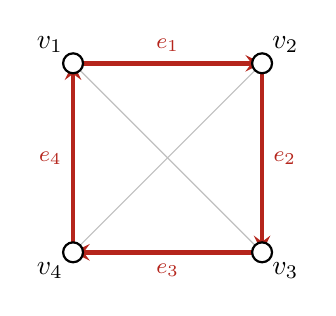
\begin{tikzpicture}[scale=1.2, thick, >=stealth]
  % \begin{ai-tikz-planner-invisible-content}
  % 1. Background: Vollständiger Graph K_4 mit dünnen grauen Kanten.
  % 2. Foreground: Der Hamilton-Kreis (v1 -> v2 -> v3 -> v4 -> v1) in dicker roter Linie.
  % 3. Nodes: Die vier Knoten v1, v2, v3, v4.
  % \end{ai-tikz-planner-invisible-content}
  
  % Coordinates
  \coordinate (V1) at (0,2);
  \coordinate (V2) at (2,2);
  \coordinate (V3) at (2,0);
  \coordinate (V4) at (0,0);
  
  % Background edges (non-cycle edges of K_4)
  \draw[gray!50, thin] (V1) -- (V3);
  \draw[gray!50, thin] (V2) -- (V4);
  
  % Hamilton Cycle (BrickRed, ultra thick)
  \draw[BrickRed, ultra thick, ->] (V1) -- (V2) node[midway, above] {\footnotesize $e_1$};
  \draw[BrickRed, ultra thick, ->] (V2) -- (V3) node[midway, right] {\footnotesize $e_2$};
  \draw[BrickRed, ultra thick, ->] (V3) -- (V4) node[midway, below] {\footnotesize $e_3$};
  \draw[BrickRed, ultra thick, ->] (V4) -- (V1) node[midway, left]  {\footnotesize $e_4$};
  
  % Nodes
  \filldraw[fill=white, draw=black] (V1) circle (3pt) node[above left] {$v_1$};
  \filldraw[fill=white, draw=black] (V2) circle (3pt) node[above right] {$v_2$};
  \filldraw[fill=white, draw=black] (V3) circle (3pt) node[below right] {$v_3$};
  \filldraw[fill=white, draw=black] (V4) circle (3pt) node[below left] {$v_4$};
\end{tikzpicture}
\end{center}
\end{math-stroke}

\subsection{Beispiele und platonische Körper}

\begin{spoken-clean}[00:35:22 - 00:36:46]
Dann noch ein Beispiel, das vielleicht noch interessant ist, bei dem man das schön hinzeichnen kann. Ich mache da noch schnell ein Bild davon. \inlinemetanote{schaltet den Projektor ein und zeigt eine Folie mit den platonischen Körpern}

Sie kennen doch die platonischen Körper, oder? Das sind die fünf regulären Polyeder --- also Polyeder, bei denen alle Seitenflächen gleich sind (zueinander kongruente regelmäßige Vielecke). Und da wissen wir, es gibt genau fünf von diesen: Tetraeder, Würfel, Oktaeder, Dodekaeder und Ikosaeder. Haben Sie wahrscheinlich einmal in der Schule oder sonst wo gesehen. Es lohnt sich, sich das mal anzuschauen. Glauben Sie mir einfach, dass es genau diese fünf gibt.

Und was wir jetzt machen können: Wir können die Kantengraphen von diesen Körpern anschauen. Das heißt, wir nehmen jetzt einfach... unsere Knoten sind die Ecken von diesen Polyedern, und die Kanten sind die (geometrischen) Kanten. Jedem von diesen platonischen Körpern können wir also einen Graphen zuordnen. Da haben wir diese fünf Graphen. Da sehen wir die Knoten und die entsprechenden Kanten dazu --- und die sind alle Hamilton-Graphen.
\end{spoken-clean}

\begin{spoken-clean}[00:36:46 - 00:38:07]
Wir sehen hier die entsprechenden Kreise: Beim Tetraeder ist das hier der Kantengraph, und dann nehmen wir einfach diesen Kreis hier --- wir sehen, er enthält alle Knoten. Oder beim Würfel können wir den Kantengraph so zeichnen, und da haben wir einen solchen Kreis (rot markierter Hamilton-Kreis). Beim Oktaeder sehen wir das auch, wenn man ihn flach auf die Ebene drückt, ist das ein planarer Graph, und da ist es dieser Kreis.

Ja, und Dodekaeder und Ikosaeder sind noch etwas komplizierter, aber man kann sie eigentlich sehr schön darstellen: Man kann sich anschaulich vorstellen, man nimmt diese Körper, macht einen dieser Kreise (eine der Begrenzungsflächen) ganz groß und drückt den Rest nach innen --- so kann man sie alle schön planar auf der Ebene zeichnen, wenn man möchte. Und da sieht man dann, dass sie alle Hamilton-Graphen sind.
\end{spoken-clean}

\begin{math-stroke}[Kantengraphen der platonischen Körper]
\begin{example}[Platonische Körper]\label[example]{ex:platonische-koerper}
Die Kantengraphen der fünf platonischen Körper (Tetraeder, Würfel, Oktaeder, Dodekaeder, Ikosaeder) sind alle Hamilton-Graphen.
\end{example}

\begin{center}
\begin{tikzpicture}[scale=1.0, thick, >=stealth]
  % \begin{ai-tikz-planner-invisible-content}
  % 1. Background: Drei repräsentative platonische Kantengraphen (Tetraeder, Würfel, Oktaeder).
  % 2. Foreground: Hamilton-Kreise in BrickRed hervorgehoben.
  % \end{ai-tikz-planner-invisible-content}

  % --- TETRAEDER ---
  \begin{scope}[shift={(0,0)}]
    \coordinate (A) at (0,1.8);
    \coordinate (B) at (-1.5,-0.6);
    \coordinate (C) at (1.5,-0.6);
    \coordinate (D) at (0,0.2);
    
    % Non-cycle edges
    \draw[gray!40, thin] (A) -- (D);
    \draw[gray!40, thin] (B) -- (C);
    
    % Hamilton Cycle
    \draw[BrickRed, ultra thick] (A) -- (B) -- (D) -- (C) -- cycle;
    
    % Nodes
    \foreach \p in {A,B,C,D} \filldraw[fill=white, draw=black] (\p) circle (2.5pt);
    \node[below=0.8cm of B, xshift=1.5cm] {\textbf{Tetraeder}};
  \end{scope}

  % --- WÜRFEL ---
  \begin{scope}[shift={(4.5,0)}]
    \coordinate (A1) at (-1.2,1.2);
    \coordinate (B1) at (1.2,1.2);
    \coordinate (C1) at (1.2,-1.2);
    \coordinate (D1) at (-1.2,-1.2);
    
    \coordinate (A2) at (-0.6,0.6);
    \coordinate (B2) at (0.6,0.6);
    \coordinate (C2) at (0.6,-0.6);
    \coordinate (D2) at (-0.6,-0.6);
    
    % Non-cycle edges
    \draw[gray!40, thin] (A1) -- (B1);
    \draw[gray!40, thin] (C1) -- (D1);
    \draw[gray!40, thin] (A2) -- (D2);
    \draw[gray!40, thin] (B2) -- (C2);
    
    % Hamilton Cycle
    \draw[BrickRed, ultra thick] (A1) -- (A2) -- (B2) -- (B1) -- (C1) -- (C2) -- (D2) -- (D1) -- cycle;
    
    % Nodes
    \foreach \p in {A1,B1,C1,D1,A2,B2,C2,D2} \filldraw[fill=white, draw=black] (\p) circle (2.5pt);
    \node[below=1.4cm of D1, xshift=1.2cm] {\textbf{Würfel}};
  \end{scope}

  % --- OKTAEDER ---
  \begin{scope}[shift={(9,0)}]
    \coordinate (U) at (0,1.5);
    \coordinate (D) at (0,-1.5);
    \coordinate (L) at (-1.5,0);
    \coordinate (R) at (1.5,0);
    \coordinate (I1) at (-0.5,-0.3);
    \coordinate (I2) at (0.5,0.3);
    
    % Non-cycle edges
    \draw[gray!40, thin] (U) -- (D);
    \draw[gray!40, thin] (L) -- (R);
    
    % Hamilton Cycle
    \draw[BrickRed, ultra thick] (U) -- (L) -- (I1) -- (D) -- (R) -- (I2) -- cycle;
    
    % Nodes
    \foreach \p in {U,D,L,R,I1,I2} \filldraw[fill=white, draw=black] (\p) circle (2.5pt);
    \node[below=1.7cm of L, xshift=1.5cm] {\textbf{Oktaeder}};
  \end{scope}
\end{tikzpicture}
\end{center}
\end{math-stroke}

\subsection{Der \texorpdfstring{$k$}{k}-dimensionale Würfel und Gray-Codes}

\begin{spoken-clean}[00:38:07 - 00:40:08]
Ein weiteres Beispiel wäre noch der Kantengraph von einem Würfel beliebiger Dimension. Das ist also noch ein weiteres Beispiel: der Kantengraph des $k$-dimensionalen Würfels (Hyperwürfels). Das ist auch ein Hamilton-Graph, und zwar für alle $k \ge \textbf{2}$. \inlinemetanote{schreibt an die Tafel}

Für $k = 2$ sehen wir: Das ist einfach das Quadrat. Ein zweidimensionaler Würfel ist ein Quadrat, und klar, da kann man einfach einmal rundherumlaufen. Das ist ein Kreis, und das ist ein Hamilton-Kreis, das ist offensichtlich.

Für $k = 3$ --- den klassischen dreidimensionalen Würfel --- müssen wir uns auch nicht sehr viel überlegen, das ist auch klar. Da kann man jetzt irgendwie laufen --- was weiß ich, zum Beispiel so: Vielleicht müssen wir eine Farbe nehmen. Man kann irgendwie so laufen, zum Beispiel so, und dann hoch, und dann rüber und nach hinten, und dann so und so und so, und da (über die verbleibenden Ecken) wieder nach vorne zum Startpunkt. Wir sehen, das gibt einen geschlossenen Kreis, und alle Knoten werden genau einmal besucht.
\end{spoken-clean}

\begin{math-stroke}[Der \texorpdfstring{$k$}{k}-dimensionale Würfel \texorpdfstring{$Q_k$}{Q\_k}]
\begin{definition}[$k$-dimensionaler Würfel]\label[definition]{def:k-dim-cube}
Der \newterm{$k$-dimensionaler Würfel} (oder Hyperwürfel) $Q_k$ ist der ungerichtete Graph, dessen Knotenmenge $V = \{0, 1\}^k$ aus allen binären Wörtern der Länge $k$ besteht. Zwei Knoten $a, b \in V$ sind genau dann durch eine Kante verbunden, wenn sie sich in genau einer Koordinate unterscheiden.
\end{definition}

\begin{center}
\begin{tikzpicture}[scale=1.4, thick, >=stealth]
  \begin{ai-tikz-planner-invisible-content}
  % 1. Background: 3D-Würfel Q_3 in sauberer Kabinett-Projektion mit gestrichelten grauen Kanten (gray!50, dashed) für Tiefenwirkung.
  % 2. Foreground Layering: Knoten werden zuerst gezeichnet, und der Hamilton-Kreis (Gray-Code: 000 -> 100 -> 110 -> 010 -> 011 -> 111 -> 101 -> 001 -> 000) wird danach als gerichtete Pfeile (BrickRed, line width=2.2pt) über die Knoten hinweg gezeichnet, wobei auf die benannten Knoten (n000 bis n111) referenziert wird. Dadurch liegen die Pfeile im Vordergrund und enden sauber an den Knotengrenzen.
  % 3. Styling: Knoten als weiße Kreise mit drop shadow, farbliche Kennzeichnung (ThemePrimary vs. ThemeSecondary) zur didaktischen Trennung der vorderen und hinteren Würfelebene.
  % 4. Labels: Eigens positionierte Textknoten mit weißer Füllung gegen Kanten-Kollisionen. Explikative Tabellen-Legende unter der Grafik.
  \end{ai-tikz-planner-invisible-content}

  % Coordinates Front Face
  \coordinate (000) at (0, 0);
  \coordinate (100) at (3.6, 0);
  \coordinate (110) at (3.6, 3.6);
  \coordinate (010) at (0, 3.6);
  
  % Coordinates Back Face (offset for clean 3D perspective)
  \coordinate (001) at (1.7, 1.5);
  \coordinate (101) at (5.3, 1.5);
  \coordinate (111) at (5.3, 5.1);
  \coordinate (011) at (1.7, 5.1);
  
  % 1. Background / Non-Hamilton Edges (Gray, dashed/subtle for depth)
  \draw[gray!50, line width=1.3pt, dashed] (000) -- (010);
  \draw[gray!50, line width=1.3pt, dashed] (100) -- (101);
  \draw[gray!50, line width=1.3pt, dashed] (110) -- (111);
  \draw[gray!50, line width=1.3pt, dashed] (001) -- (011);
  
  % 2. Vertices (Styled as clean circles with shadows) - Drawn BEFORE the Hamilton cycle path
  % Back vertices first (for proper layering)
  \node (n001) [circle, draw=ThemeSecondary, fill=white, line width=1.2pt, inner sep=3pt, drop shadow] at (001) {};
  \node (n101) [circle, draw=ThemeSecondary, fill=white, line width=1.2pt, inner sep=3pt, drop shadow] at (101) {};
  \node (n111) [circle, draw=ThemeSecondary, fill=white, line width=1.2pt, inner sep=3pt, drop shadow] at (111) {};
  \node (n011) [circle, draw=ThemeSecondary, fill=white, line width=1.2pt, inner sep=3pt, drop shadow] at (011) {};
  
  % Front vertices
  \node (n000) [circle, draw=ThemePrimary, fill=white, line width=1.4pt, inner sep=3.2pt, drop shadow] at (000) {};
  \node (n100) [circle, draw=ThemePrimary, fill=white, line width=1.4pt, inner sep=3.2pt, drop shadow] at (100) {};
  \node (n110) [circle, draw=ThemePrimary, fill=white, line width=1.4pt, inner sep=3.2pt, drop shadow] at (110) {};
  \node (n010) [circle, draw=ThemePrimary, fill=white, line width=1.4pt, inner sep=3.2pt, drop shadow] at (010) {};
  
  % 3. Hamilton Cycle / Gray-Code Path in Foreground (BrickRed, bold, with directional arrows)
  % Back face part of cycle: 010 -> 011 -> 111 -> 101 -> 001 -> 000
  \draw[->, BrickRed, line width=2.2pt] (n010) -- (n011);
  \draw[->, BrickRed, line width=2.2pt] (n011) -- (n111);
  \draw[->, BrickRed, line width=2.2pt] (n111) -- (n101);
  \draw[->, BrickRed, line width=2.2pt] (n101) -- (n001);
  \draw[->, BrickRed, line width=2.2pt] (n001) -- (n000);
  
  % Front face part of cycle: 000 -> 100 -> 110 -> 010
  \draw[->, BrickRed, line width=2.2pt] (n000) -- (n100);
  \draw[->, BrickRed, line width=2.2pt] (n100) -- (n110);
  \draw[->, BrickRed, line width=2.2pt] (n110) -- (n010);
  
  % 4. Labels with custom offsets and white backgrounds to prevent line overlap
  \node[font=\sffamily\footnotesize\bfseries, text=ThemeSecondary, fill=white, inner xsep=2pt, inner ysep=1pt, rounded corners=2pt] at ($(001)+(-0.35,0.25)$) {$001$};
  \node[font=\sffamily\footnotesize\bfseries, text=ThemeSecondary, fill=white, inner xsep=2pt, inner ysep=1pt, rounded corners=2pt] at ($(101)+(0.4,-0.2)$) {$101$};
  \node[font=\sffamily\footnotesize\bfseries, text=ThemeSecondary, fill=white, inner xsep=2pt, inner ysep=1pt, rounded corners=2pt] at ($(111)+(0.4,0.25)$) {$111$};
  \node[font=\sffamily\footnotesize\bfseries, text=ThemeSecondary, fill=white, inner xsep=2pt, inner ysep=1pt, rounded corners=2pt] at ($(011)+(-0.35,0.25)$) {$011$};
  
  \node[font=\sffamily\footnotesize\bfseries, text=ThemePrimary, fill=white, inner xsep=2pt, inner ysep=1pt, rounded corners=2pt] at ($(000)+(-0.4,-0.3)$) {$000$};
  \node[font=\sffamily\footnotesize\bfseries, text=ThemePrimary, fill=white, inner xsep=2pt, inner ysep=1pt, rounded corners=2pt] at ($(100)+(0.4,-0.3)$) {$100$};
  \node[font=\sffamily\footnotesize\bfseries, text=ThemePrimary, fill=white, inner xsep=2pt, inner ysep=1pt, rounded corners=2pt] at ($(110)+(0.4,0.3)$) {$110$};
  \node[font=\sffamily\footnotesize\bfseries, text=ThemePrimary, fill=white, inner xsep=2pt, inner ysep=1pt, rounded corners=2pt] at ($(010)+(-0.4,0.3)$) {$010$};
  
  % 5. Explanatory Legend / Caption badge below
  \node[draw=ThemePrimary!60, fill=ThemeBgLight, rounded corners=4pt, inner xsep=10pt, inner ysep=6pt, font=\sffamily\small, drop shadow] at (2.65, -1.2) {
    \begin{tabular}{c}
      \textbf{\textcolor{BrickRed}{Roter Pfeilpfad:}} Hamilton-Kreis im $Q_3$ \\
      \footnotesize Zyklischer Gray-Code: $000 \to 100 \to 110 \to 010 \to 011 \to 111 \to 101 \to 001 \to 000$
    \end{tabular}
  };
\end{tikzpicture}
\end{center}
\end{math-stroke}

\begin{spoken-clean}[00:41:24 - 00:42:44]
Okay, und für beliebiges $k$ müssen wir uns das wie folgt vorstellen: Wir schauen uns jetzt den $k$-dimensionalen Würfel an. Wir betrachten im $\mathbb{R}^k$ all die Punkte --- die Knoten sind genau die Punkte, bei denen alle Koordinaten aus Nullen und Einsen bestehen.

Und zwei davon sind genau dann verbunden, wenn sie sich in genau einer (Koordinaten-)Stelle unterscheiden. Das ist unser Würfel. Das heißt, wir identifizieren die... wie viele Ecken hat eigentlich ein $k$-dimensionaler Würfel? Ja?
\end{spoken-clean}

\begin{student-interaction}[Student Answer]
$2^k$.
\end{student-interaction}

\begin{spoken-clean}[00:42:44 - 00:43:45]
$2^k$, genau. Wir identifizieren die $2^k$ Ecken des $k$-dimensionalen Würfels mit binären Wörtern der Länge $k$. Was ist ein binäres Wort? Das ist einfach ein Wort bestehend aus Nullen und Einsen --- also die Elemente in $\{0, 1\}^k$.

Und zwei solche Wörter $a$ und $b$ sind durch eine Kante verbunden, falls sie sich in genau einer Stelle unterscheiden. Okay. Und wir schauen uns dann nach der Pause an, weshalb daraus folgt beziehungsweise weshalb das zeigt, dass es immer einen Hamilton-Kreis im $k$-dimensionalen Würfel gibt. Gut, wir machen in einer Viertelstunde weiter.
\end{spoken-clean}

\begin{lecture-break}[Vorlesungspause]
Der Dozent kündigt eine 15-minütige Pause an. Das Video wird nach der Pause bei Zeitstempel 00:43:45 fortgesetzt.
\end{lecture-break}

\subsection{Gray-Codes}

\begin{spoken-clean}[00:43:45 - 00:46:50]
Also, wir haben hier unseren $k$-dimensionalen Würfel. Und wir wollen zeigen, dass dieser Kantengraph hier ein Hamilton-Graph ist. Das folgt aus der folgenden Behauptung, die wir beweisen werden. Was sagt diese Behauptung? Sie sagt:

Es gibt eine zyklische Folge --- nennen wir sie $a_1$ bis $a_{2^k}$ --- aus den $2^k$ verschiedenen binären Wörtern der Länge $k$, sodass sich $a_\ell$ und $a_{\ell+1}$ für $\ell = 1$ bis $2^k - 1$ sowie $a_{2^k}$ und $a_1$ in genau einer Stelle unterscheiden.

Wir müssen also zeigen, dass eine solche Folge existiert, bei der wir immer nur ein Bit wechseln und am Schluss wieder am Anfang ankommen. Eine solche Folge nennt man einen Gray-Code.

Okay. Ich weiß nicht Genaueres darüber, weshalb das Gray-Code heißt. Das kommt wahrscheinlich historisch aus der Codierungstheorie, in der man untersucht, wie man Wörter gut wählt, um Informationen verlässlich zu übermitteln --- fehlerkorrigierende Codes und so weiter. Aber das ist für uns an dieser Stelle nicht so wichtig; wichtig ist für uns nur der mathematische Beweis, dass es eine solche Folge für jede Dimension $k$ immer gibt.

Und der Beweis ist erfreulich einfach, das ist einfach vollständige Induktion nach $k$.
\end{spoken-clean}

\begin{math-stroke}[Existenz von Gray-Codes]
\begin{proposition}[Existenz von Gray-Codes]\label[proposition]{prop:gray-code-existenz}
Für jedes $k \ge 1$ existiert eine zyklische Folge $(a_1, \dots, a_{2^k})$ aller $2^k$ verschiedenen binären Wörter der Länge $k$, sodass sich aufeinanderfolgende Wörter $a_{\ell}$ und $a_{\ell+1}$ (sowie das letzte Wort $a_{2^k}$ und das erste Wort $a_1$) in genau einer Stelle unterscheiden. Ein solcher Zyklus entspricht genau einem Hamilton-Kreis im Hyperwürfel $Q_k$.
\end{proposition}
\end{math-stroke}

\begin{proof}[Beweis der Existenz von Gray-Codes]
\begin{spoken-clean}[00:46:50 - 00:48:18]
Der Induktionsanfang für $k=1$: Okay, da ist die Sache klar (trivial). Da nehmen wir einfach die Folge $(0, 1)$, und das war's. (Die beiden Wörter unterscheiden sich in genau einer Stelle, und der Rückweg von $1$ zu $0$ ebenfalls.) Das ist der Induktionsanfang, völlig trivial.

Für den Induktionsschritt von $k$ auf $k+1$ nehmen wir an, dass so ein Gray-Code existiert. Schreiben wir den mal hin: Das ist eine Folge $(a_1, \dots, a_{2^k})$. Und daraus bauen wir jetzt ganz einfach einen Gray-Code für $k+1$. \inlinemetanote{schreibt an die Tafel}
\end{spoken-clean}

\begin{spoken-clean}[00:48:18 - 00:49:28]
Wir machen das wie folgt: Zuerst nehmen wir diesen ganzen Code und setzen überall eine $0$ voran. Das heißt, unsere ersten $2^k$ Wörter sind $(0a_1, 0a_2, \dots, 0a_{2^k})$. \inlinemetanote{schreibt an die Tafel} Das sind einfach Wörter, und wir haben überall eine $0$ vorangestellt.
\end{spoken-clean}

\begin{spoken-clean}[00:49:28 - 00:50:58]
Das bildet jetzt schon mal eine sehr gute Folge, weil die sich immer in einer Stelle unterscheiden --- die $a_i$ unterscheiden sich in einer Stelle, und die vorangestellte $0$ bleibt ja immer $0$. Das heißt, die aufeinanderfolgenden Wörter hier unterscheiden sich auch immer nur in einer Stelle.

Als nächstes Element in meiner Folge nehme ich jetzt das Element $1a_{2^k}$. Was muss ich da wechseln? Ich muss einfach aus der $0$ vorne eine $1$ machen, und der Rest, das Wort $a_{2^k}$, bleibt gleich. Das heißt, das unterscheidet sich (vom vorherigen Wort $0a_{2^k}$) auch nur in einer (einzigen) Stelle. \inlinemetanote{schreibt an die Tafel}

Und jetzt laufe ich den ganzen Code nochmals ab, aber ich laufe ihn rückwärts ab! Ich hänge also jetzt hinten dran: $1a_{2^k-1}, 1a_{2^k-2}$ und so weiter, bis ich am Schluss bei $1a_1$ bin. (Anschließend spiegeln wir die restliche Folge und stellen jeweils eine $1$ voran). Das ist meine ganze Folge: zuerst überall eine $0$ voranstellen und vorwärts durchlaufen, dann aus der vordersten $0$ eine $1$ machen und denselben Code rückwärts zurücklaufen. \inlinemetanote{schreibt an die Tafel}
\end{spoken-clean}

\begin{spoken-clean}[00:50:58 - 00:52:40]
Ist das ein Gray-Code? Ja, also hier unterscheiden sich immer alle um eins. Die hier unterscheiden sich um eins. Die hier auch --- weil sich aufeinanderfolgende Wörter im Gray-Code in einer Stelle unterscheiden und die vorangestellte $1$ unverändert bleibt. Das ist hier also auch gegeben.

Und jetzt bleibt nur noch der Schritt zurück, vom Ende zum Anfang. Das heißt, ich bin jetzt bei $1a_1$, und ich muss zurück zu $0a_1$. Geht das? Na klar, ich muss einfach aus der ersten $1$ eine $0$ machen, das heißt, ich kippe auch hier wieder genau ein einziges Bit um. Damit haben wir bewiesen: Für alle Dimensionen existiert ein gültiger Gray-Code für $k+1$. \inlinemetanote{schreibt an die Tafel}
\end{spoken-clean}

\begin{math-stroke}
Wir führen den Beweis per vollständiger Induktion nach der Dimension $k$:
\begin{itemize}
    \item \textbf{Induktionsanfang ($k=1$):} Die Folge $(a_1, a_2) := (0, 1)$ ist ein zyklischer Gray-Code der Länge $2^1 = 2$, da sich $0$ und $1$ in genau einer Stelle unterscheiden.
    \item \textbf{Induktionsschritt ($k \to k+1$):} Sei $(a_1, a_2, \dots, a_{2^k})$ ein zyklischer Gray-Code der Länge $2^k$. Wir konstruieren eine neue Folge $(b_1, \dots, b_{2^{k+1}})$ der Länge $2^{k+1}$ durch Spiegelung und Voranstellen von $0$ bzw. $1$:
    \[
    b_i := \begin{cases}
    0a_i & \text{für } 1 \le i \le 2^k \\
    1a_{2^{k+1} - i + 1} & \text{für } 2^k + 1 \le i \le 2^{k+1}
    \end{cases}
    \]
    Wir verifizieren die Gray-Code-Eigenschaften für die Übergänge:
    \begin{enumerate}[label=\textbf{(\arabic*)}]
        \item \textbf{Innerhalb der ersten Hälfte ($1 \le i < 2^k$):} $b_i = 0a_i$ und $b_{i+1} = 0a_{i+1}$ unterscheiden sich nur in einer Stelle, da sich $a_i$ und $a_{i+1}$ nach Induktionsvoraussetzung nur in einer Stelle unterscheiden.
        \item \textbf{Am Übergangspunkt ($i = 2^k$):} $b_{2^k} = 0a_{2^k}$ und $b_{2^k+1} = 1a_{2^k}$ unterscheiden sich exakt nur in der ersten (vorangestellten) Stelle.
        \item \textbf{Innerhalb der zweiten Hälfte ($2^k + 1 \le i < 2^{k+1}$):} $b_i = 1a_{2^{k+1}-i+1}$ und $b_{i+1} = 1a_{2^{k+1}-i}$ unterscheiden sich analog zur ersten Hälfte nur in einer Stelle.
        \item \textbf{Am zyklischen Rücklauf ($i = 2^{k+1}$):} Das letzte Element $b_{2^{k+1}} = 1a_1$ und das erste Element $b_1 = 0a_1$ unterscheiden sich ebenfalls exakt nur in der ersten Stelle.
    \end{enumerate}
    Die konstruierte Folge ist somit ein wohldefinierter, zyklischer Gray-Code der Länge $2^{k+1}$.
\end{itemize}
\end{math-stroke}
\end{proof}

\subsection{Der vierdimensionale Hyperwürfel}

\begin{spoken-clean}[00:52:40 - 00:54:38]
Das ist hier auch noch ein schönes Beispiel. Sie können sich vorstellen, diese Hyperwürfel kriegen sehr schnell sehr viele Ecken. (Ein eindimensionaler Würfel hat $2$ Ecken, ein zweidimensionaler $4$, ein dreidimensionaler $8$, und der vierdimensionale Würfel besitzt bereits $16$ Ecken.) Das hat dann im vierdimensionalen schon $16$ Ecken und so weiter. Und das ist geometrisch nicht mehr so einfach zu visualisieren --- Sie kennen das sicher, das ist so das Modell für die vierte Dimension.

Das ist jetzt dieses Bildchen hier auf der Folie. Das ist der vierdimensionale Würfel, sein Kantengraph. Und diese Linie ist ein solcher Hamilton-Kreis (ein möglicher Gray-Code) --- Sie sehen ihn da fett rot eingezeichnet in dem Graph. (Man sieht sehr schön: Von einem Wort zum nächsten verändert sich immer nur genau eine Koordinate, das heißt, wir bewegen uns immer exakt entlang einer Kante.) Und wenn Sie wollen, können Sie ja mal nachprüfen, ob das stimmt und dieser Weg tatsächlich jeden der $16$ Knoten genau einmal besucht.

Okay, gut, damit haben wir einige schöne Beispiele gesehen. Jetzt wollen wir uns fragen --- weil wir ja gesehen haben, dass man im Allgemeinen nicht so einfach entscheiden kann, ob ein Hamilton-Kreis existiert oder nicht --- gibt es vielleicht trotzdem ein paar Kriterien? Und da gibt es den Satz von Dirac, den ich Ihnen jetzt noch vorstellen möchte. Zuerst wische ich aber noch die Tafel.
\end{spoken-clean}

\begin{meta-note}[Tafelreinigung]
Der Dozent wischt die Tafel gründlich, um Platz für das nächste Thema zu schaffen, während auf dem Projektor eine Folie des vierdimensionalen Hyperwürfels ($Q_4$, Tesseract) mit einem rot markierten Hamilton-Kreis zu sehen ist.
\end{meta-note}

% \begin{math-stroke}[Der vierdimensionale Hyperwürfel \texorpdfstring{$Q_4$}{Q\_4}]
% \begin{center}
% \begin{tikzpicture}[scale=1.5, thick, >=stealth]
%   % \begin{ai-tikz-planner-invisible-content}
%   % 1. Background: Projektion des Tesseracts (Q_4) mit dünnen grauen Linien.
%   % 2. Foreground: Ein Hamilton-Kreis (Gray-Code) in dicker roter Linie (BrickRed).
%   % \end{ai-tikz-planner-invisible-content}
  
%   % Inner Cube Coordinates
%   \coordinate (0000) at (-0.5,-0.5,-0.5);
%   \coordinate (1000) at (0.5,-0.5,-0.5);
%   \coordinate (1100) at (0.5,0.5,-0.5);
%   \coordinate (0100) at (-0.5,0.5,-0.5);
%   \coordinate (0010) at (-0.3,-0.3,0.5);
%   \coordinate (1010) at (0.7,-0.3,0.5);
%   \coordinate (1110) at (0.7,0.7,0.5);
%   \coordinate (0110) at (-0.3,0.7,0.5);
  
%   % Outer Cube Coordinates
%   \coordinate (0001) at (-1.5,-1.5,-1.5);
%   \coordinate (1001) at (1.5,-1.5,-1.5);
%   \coordinate (1101) at (1.5,1.5,-1.5);
%   \coordinate (0101) at (-1.5,1.5,-1.5);
%   \coordinate (0011) at (-1.0,-1.0,1.5);
%   \coordinate (1011) at (2.0,-1.0,1.5);
%   \coordinate (1111) at (2.0,2.0,1.5);
%   \coordinate (0111) at (-1.0,2.0,1.5);

%   % Non-cycle edges (gray, thin)
%   \draw[gray!30, thin] (0000) -- (1000);
%   \draw[gray!30, thin] (1100) -- (0100);
%   \draw[gray!30, thin] (0010) -- (1010);
%   \draw[gray!30, thin] (1110) -- (0110);
%   \draw[gray!30, thin] (0001) -- (1001);
%   \draw[gray!30, thin] (1101) -- (0101);
%   \draw[gray!30, thin] (0011) -- (1011);
%   \draw[gray!30, thin] (1111) -- (0111);
%   \draw[gray!30, thin] (0000) -- (0001);
%   \draw[gray!30, thin] (1000) -- (1001);
%   \draw[gray!30, thin] (1100) -- (1101);
%   \draw[gray!30, thin] (0100) -- (0101);
%   \draw[gray!30, thin] (0010) -- (0011);
%   \draw[gray!30, thin] (1010) -- (1011);
%   \draw[gray!30, thin] (1110) -- (1111);
%   \draw[gray!30, thin] (0110) -- (0111);

%   % Hamilton Cycle (BrickRed, ultra thick)
%   \draw[BrickRed, ultra thick] (0000) -- (0100) -- (0110) -- (0010) -- (0011) -- (0111) -- (0101) -- (0001) -- (1001) -- (1000) -- (1100) -- (1101) -- (1111) -- (1011) -- (1010) -- (1110) -- cycle;

%   % Nodes (small dots)
%   \foreach \p in {0000,1000,1100,0100,0010,1010,1110,0110,0001,1001,1101,0101,0011,1011,1111,0111}
%     \filldraw[fill=white, draw=black] (\p) circle (2pt);
% \end{tikzpicture}
% \end{center}
% \end{math-stroke}


\begin{math-stroke}[Der vierdimensionale Hyperwürfel \texorpdfstring{$Q_4$}{Q\_4}]
\begin{center}
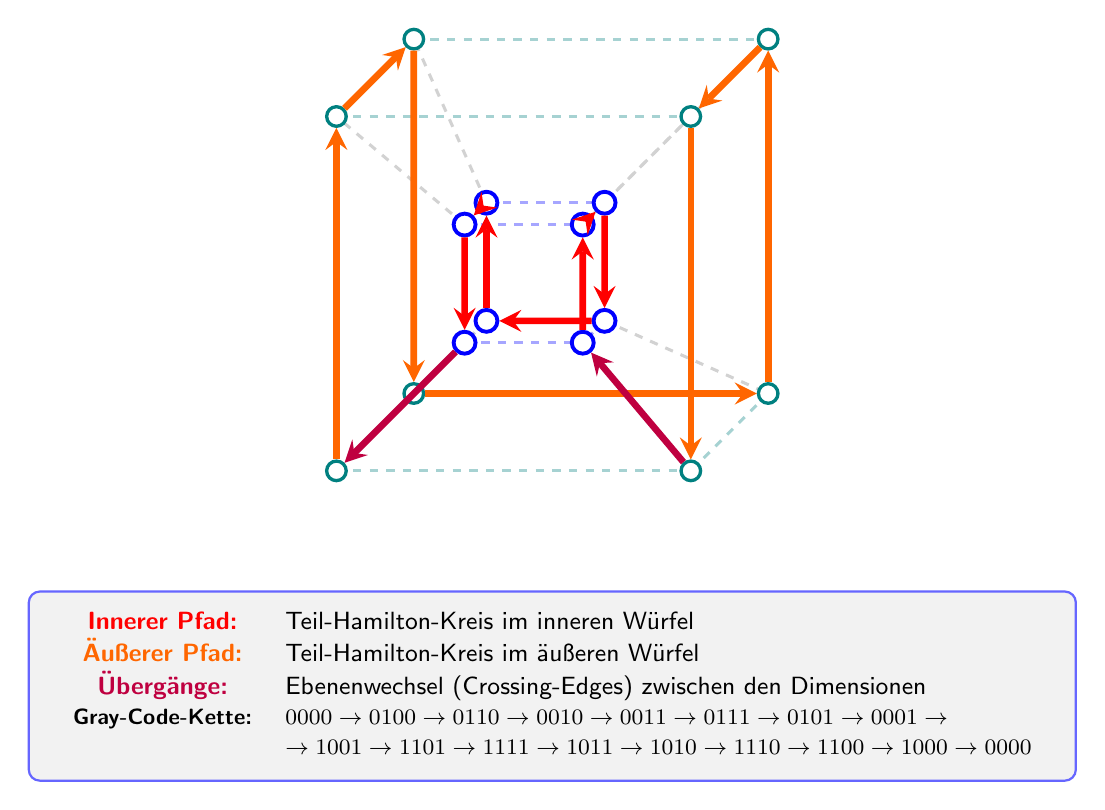
\begin{tikzpicture}[scale=1.5, thick, >=stealth]
  % \begin{ai-tikz-planner-invisible-content}
  % 1. Background: Projektion des Tesseracts (Q_4) mit strukturell getrennten Dimensionen. Der innere 3D-Würfel ist in Blau (blue) gezeichnet, der äußere in Teal (teal).
  % 2. Visual Hierarchy: Nicht-zyklische Kanten sind dünn, gestrichelt und farblich dezent gehalten (blue!35 bzw. teal!35).
  % 3. Foreground Layering & Shading: Ecken werden zuerst als benannte Kreise (n0000 bis n1111) gezeichnet. Der rote Pfad (Hamilton-Kreis / Gray-Code) wird danach im Vordergrund über die Ecken gelegt. Der Pfad ist farblich schattiert (red im inneren Würfel, orange!80!red im äußeren Würfel, purple für die Ebenen-Wechsel-Übergänge).
  % 4. Legend: Eine detaillierte Legende am Fuß der Grafik erklärt den Farbcode und den mathematisch korrekten 4-Bit Gray-Code.
  % \end{ai-tikz-planner-invisible-content}
  
  % Inner Cube Coordinates
  \coordinate (0000) at (-0.5,-0.5,-0.5);
  \coordinate (1000) at (0.5,-0.5,-0.5);
  \coordinate (1100) at (0.5,0.5,-0.5);
  \coordinate (0100) at (-0.5,0.5,-0.5);
  \coordinate (0010) at (-0.3,-0.3,0.5);
  \coordinate (1010) at (0.7,-0.3,0.5);
  \coordinate (1110) at (0.7,0.7,0.5);
  \coordinate (0110) at (-0.3,0.7,0.5);
  
  % Outer Cube Coordinates
  \coordinate (0001) at (-1.5,-1.5,-1.5);
  \coordinate (1001) at (1.5,-1.5,-1.5);
  \coordinate (1101) at (1.5,1.5,-1.5);
  \coordinate (0101) at (-1.5,1.5,-1.5);
  \coordinate (0011) at (-1.0,-1.0,1.5);
  \coordinate (1011) at (2.0,-1.0,1.5);
  \coordinate (1111) at (2.0,2.0,1.5);
  \coordinate (0111) at (-1.0,2.0,1.5);

  % 1. Non-cycle edges (dashed, thin)
  % Inner Cube (blue!35)
  \draw[blue!35, dashed, line width=1.1pt] (0000) -- (1000);
  \draw[blue!35, dashed, line width=1.1pt] (0100) -- (1100);
  \draw[blue!35, dashed, line width=1.1pt] (0010) -- (1010);
  \draw[blue!35, dashed, line width=1.1pt] (0110) -- (1110);
  \draw[blue!35, dashed, line width=1.1pt] (0000) -- (0010);
  \draw[blue!35, dashed, line width=1.1pt] (1000) -- (1010);
  
  % Outer Cube (teal!35)
  \draw[teal!35, dashed, line width=1.1pt] (0001) -- (1001);
  \draw[teal!35, dashed, line width=1.1pt] (0101) -- (1101);
  \draw[teal!35, dashed, line width=1.1pt] (0011) -- (1011);
  \draw[teal!35, dashed, line width=1.1pt] (0111) -- (1111);
  \draw[teal!35, dashed, line width=1.1pt] (0001) -- (0011);
  \draw[teal!35, dashed, line width=1.1pt] (1001) -- (1011);
  
  % Connecting Edges (gray!35)
  \draw[gray!35, dashed, line width=1.1pt] (0000) -- (0001);
  \draw[gray!35, dashed, line width=1.1pt] (1000) -- (1001);
  \draw[gray!35, dashed, line width=1.1pt] (1100) -- (1101);
  \draw[gray!35, dashed, line width=1.1pt] (0100) -- (0101);
  \draw[gray!35, dashed, line width=1.1pt] (1110) -- (1111);
  \draw[gray!35, dashed, line width=1.1pt] (0110) -- (0111);

  % 2. Vertices (Styled circles) - Drawn BEFORE the cycle paths
  % Outer Cube Ecken (teal)
  \foreach \p in {0001,1001,1101,0101,0011,1011,1111,0111}
    \node (n\p) [circle, draw=teal, fill=white, line width=1.2pt, inner sep=2.5pt] at (\p) {};
    
  % Inner Cube Ecken (blue)
  \foreach \p in {0000,1000,1100,0100,0010,1010,1110,0110}
    \node (n\p) [circle, draw=blue, fill=white, line width=1.4pt, inner sep=2.8pt] at (\p) {};

  % 3. Hamilton Cycle / Gray-Code Path in Foreground (Bold, colored by dimension/transition)
  % Inner Cube Path segments (red)
  \draw[->, red, line width=2.4pt] (n0000) -- (n0100);
  \draw[->, red, line width=2.4pt] (n0100) -- (n0110);
  \draw[->, red, line width=2.4pt] (n0110) -- (n0010);
  
  \draw[->, red, line width=2.4pt] (n1010) -- (n1110);
  \draw[->, red, line width=2.4pt] (n1110) -- (n1100);
  \draw[->, red, line width=2.4pt] (n1100) -- (n1000);
  \draw[->, red, line width=2.4pt] (n1000) -- (n0000);

  % Outer Cube Path segments (orange!80!red)
  \draw[->, orange!80!red, line width=2.4pt] (n0011) -- (n0111);
  \draw[->, orange!80!red, line width=2.4pt] (n0111) -- (n0101);
  \draw[->, orange!80!red, line width=2.4pt] (n0101) -- (n0001);
  \draw[->, orange!80!red, line width=2.4pt] (n0001) -- (n1001);
  \draw[->, orange!80!red, line width=2.4pt] (n1001) -- (n1101);
  \draw[->, orange!80!red, line width=2.4pt] (n1101) -- (n1111);
  \draw[->, orange!80!red, line width=2.4pt] (n1111) -- (n1011);

  % Crossing / Transition Path segments (purple)
  \draw[->, purple, line width=2.4pt] (n0010) -- (n0011);
  \draw[->, purple, line width=2.4pt] (n1011) -- (n1010);

  % 4. Explanatory Legend / Caption badge below
  \node[draw=blue!60, fill=gray!10, rounded corners=4pt, inner xsep=10pt, inner ysep=6pt, font=\sffamily\small] at (0.25, -3.4) {
    \begin{tabular}{cl}
      \textbf{\textcolor{red}{Innerer Pfad:}} & Teil-Hamilton-Kreis im inneren Würfel \\
      \textbf{\textcolor{orange!80!red}{Äußerer Pfad:}} & Teil-Hamilton-Kreis im äußeren Würfel \\
      \textbf{\textcolor{purple}{Übergänge:}} & Ebenenwechsel (Crossing-Edges) zwischen den Dimensionen \\
      \footnotesize \textbf{Gray-Code-Kette:} & \footnotesize $0000 \to 0100 \to 0110 \to 0010 \to 0011 \to 0111 \to 0101 \to 0001 \to {}$ \\
      & \footnotesize $\to 1001 \to 1101 \to 1111 \to 1011 \to 1010 \to 1110 \to 1100 \to 1000 \to 0000$
    \end{tabular}
  };
\end{tikzpicture}
\end{center}
\end{math-stroke}



\begin{spoken-clean}[00:54:38 - 00:56:52]
Solche Würfelstrukturen sind in vielen Bereichen der modernen Mathematik von großer Bedeutung. In der geometrischen Gruppentheorie war es in den letzten Jahren beispielsweise sehr populär, sogenannte kubische Komplexe zu untersuchen. Dabei nimmt man Würfel verschiedener Dimensionen, klebt sie nach bestimmten geometrischen Regeln zusammen und erhält dadurch mächtige Werkzeuge, um abstrakte Gruppen über die Kantengraphen dieser Komplexe zu studieren.

Das ist natürlich nicht Teil dieser Vorlesung, aber es war für einige Jahre mein persönliches Steckenpferd, diese kubischen Komplexe auf mathematische Gruppen anzuwenden.
\end{spoken-clean}

\section{Bipartite Graphen}

\subsection{Das Konzept bipartiter Graphen}

\begin{spoken-clean}[00:56:52 - 00:58:30]
Als letztes Thema möchte ich heute noch den sogenannten Heiratssatz besprechen, obwohl das ein sehr unglücklicher Name ist. Zuvor noch eine Definition, die auch auf dem Übungsblatt vorkommt: Ein Graph heißt bipartit. Bipartit ist ein lustiges Wort. Was heißt das? Man kann den Graphen in zwei Teile teilen, also man kann die Knotenmenge so in zwei verschiedene (disjunkte) Mengen aufteilen, sodass alle Kanten ausschließlich zwischen der einen Menge und der anderen Menge verlaufen.

Er heißt also formal bipartit, falls $V$ die disjunkte Vereinigung von zwei Teilmengen $U$ und $W$ ist --- disjunkte Vereinigung bedeutet, dass $V = U \cup W$ ist und der Durchschnitt $U \cap W = \emptyset$ leer ist.
\end{spoken-clean}

\begin{math-stroke}
\begin{definition}[Bipartiter Graph]\label[definition]{def:bipartit}
Ein ungerichteter Graph $G = (V, E)$ heißt \newterm{bipartit}, falls sich seine Knotenmenge $V$ als disjunkte Vereinigung zweier Teilmengen $U$ und $W$ darstellen lässt:
\[
V = U \;\dot{\cup}\; W \quad (\text{d.\,h. } V = U \cup W \text{ und } U \cap W = \emptyset)
\]
sodass alle Kanten in $E$ ausschließlich zwischen $U$ und $W$ verlaufen:
\[
E \subseteq \bigl\{ \{u, w\} \;\big|\; u \in U, w \in W \bigr\}
\]
Wir schreiben einen solchen Graphen auch als Tripel $G = (U, W, E)$.
\end{definition}

\begin{center}
\begin{tikzpicture}[scale=1.2, thick, >=stealth]
  % \begin{ai-tikz-planner-invisible-content}
  % 1. Background: Bipartiter Graph mit zwei disjunkten Spalten U und W.
  % 2. Foreground: Kanten, die ausschließlich zwischen U und W verlaufen (keine internen Kanten).
  % \end{ai-tikz-planner-invisible-content}
  
  % Column U (ForestGreen)
  \coordinate (U1) at (0,2.5);
  \coordinate (U2) at (0,1.5);
  \coordinate (U3) at (0,0.5);
  
  % Column W (MidnightBlue)
  \coordinate (W1) at (3,2.5);
  \coordinate (W2) at (3,1.5);
  \coordinate (W3) at (3,0.5);
  
  % Edges
  \draw (U1) -- (W1);
  \draw (U1) -- (W2);
  \draw (U2) -- (W2);
  \draw (U2) -- (W3);
  \draw (U3) -- (W1);
  \draw (U3) -- (W3);
  
  % Nodes
  \filldraw[fill=white, draw=black] (U1) circle (3pt) node[left] {$u_1$};
  \filldraw[fill=white, draw=black] (U2) circle (3pt) node[left] {$u_2$};
  \filldraw[fill=white, draw=black] (U3) circle (3pt) node[left] {$u_3$};
  
  % Nodes (W)
  \filldraw[fill=white, draw=black] (W1) circle (3pt) node[right] {$w_1$};
  \filldraw[fill=white, draw=black] (W2) circle (3pt) node[right] {$w_2$};
  \filldraw[fill=white, draw=black] (W3) circle (3pt) node[right] {$w_3$};
  
  % Labels
  \node[above=0.3cm of U1, ForestGreen, font=\bfseries] {$U$};
  \node[above=0.3cm of W1, MidnightBlue, font=\bfseries] {$W$};
\end{tikzpicture}
\end{center}
\end{math-stroke}

\begin{spoken-clean}[00:58:30 - 00:59:56]
...sodass die Kanten alle in der Menge $U \times W$ enthalten sind (was natürlich eine Teilmenge von $V \times V$ ist). Wir schreiben den Graphen dann einfach als $G = (U, W, E)$.

Okay, wenn wir also sagen, $G$ ist ein bipartiter Graph und wir schreiben ihn so, dann heißt das: Das eine ist die eine Knotenmenge ($U$), das andere die andere ($W$), und die Kanten gehen alle von Elementen hier zu Elementen da. 

Es gibt natürlich Graphen, die nicht bipartit sind --- das ist eine sehr spezielle Struktur (Klasse von Graphen), die meisten sind es im Allgemeinen natürlich nicht.
\end{spoken-clean}

% --- TEIL 3 ---

\subsection{Bipartite Graphen und Färbbarkeit}

\begin{math-stroke}
\begin{theorem}[Zwei-Färbbarkeit bipartiter Graphen]\label[theorem]{thm:bipartit-faerbbarkeit}
Ein ungerichteter Graph $G = (V, E)$ ist genau dann bipartit, wenn er zwei-färbbar ist. Das bedeutet, es existiert eine Färbungsfunktion $c \colon V \to \{\text{Rot}, \text{Blau}\}$, sodass für alle Kanten $\{u, v\} \in E$ gilt:
\[
c(u) \neq c(v).
\]
\end{theorem}

\begin{explanation-of-steps}[Bedeutung der Zwei-Färbbarkeit]
In einem bipartiten Graphen $G = (U, W, E)$ können wir allen Knoten in $U$ die Farbe Rot und allen Knoten in $W$ die Farbe Blau zuweisen. Da per Definition alle Kanten ausschließlich zwischen $U$ und $W$ verlaufen, gibt es keine Kanten zwischen gleichfarbigen Knoten. Dies zeigt die Äquivalenz zur Zwei-Färbbarkeit.
\end{explanation-of-steps}
\end{math-stroke}

\begin{spoken-clean}[00:59:56 - 01:01:08]
Es gibt dazu noch eine Übungsaufgabe, in der wir uns eine Verallgemeinerung davon anschauen, nämlich die Frage, wie ein Graph färbbar ist. Ein Graph ist genau dann bipartit, wenn er zweifärbbar ist. Das heißt, man kann allen Knoten eine Farbe --- blau oder rot --- geben, sodass nie zwei gleichfarbige Knoten durch eine Kante verbunden sind (d.\,h.\ es geht nie eine Kante von einem roten Knoten zu einem roten Knoten, sondern immer nur zu einem blauen). Gut, okay, das sind bipartite Graphen.

Bipartite Graphen treten natürlich in der Praxis erstaunlich häufig auf. Was weiß ich, wenn man zum Beispiel Brieffreunde zwischen Europa und Amerika betrachtet: Die Personen sind entweder in Europa oder in Amerika ansässig, aber sie schreiben sich Briefe nur über den Atlantik hinweg. Das wäre ein klassischer bipartiter Graph.
\end{spoken-clean}

\begin{math-stroke}[Beispiel eines bipartiten Graphen]
\begin{example}[Brieffreunde-Netzwerk]\label[example]{ex:brieffreunde}
Betrachte das Netzwerk von Brieffreunden zwischen Europa und Amerika. Wir definieren den Graphen $G = (U, W, E)$ durch:
\begin{itemize}
    \item \textbf{$U$:} Die Menge der Personen in Europa.
    \item \textbf{$W$:} Die Menge der Personen in Amerika.
    \item \textbf{$E$:} Die Menge der Kanten, wobei $\{u, w\} \in E$ bedeutet, dass $u \in U$ und $w \in W$ Brieffreunde sind.
\end{itemize}
Da Briefe nur über den Atlantik geschickt werden (keine Brieffreundschaften innerhalb Europas oder innerhalb Amerikas), ist dieser Graph bipartit.
\end{example}
\end{math-stroke}

\begin{spoken-clean}[01:01:08 - 01:02:13]
Das heißt, bei bipartiten Graphen spielt es oft keine so große Rolle mehr, ob sie gerichtet oder ungerichtet sind. Man weiß eigentlich für jede Kante genau, ob sie in $U$ anfängt und in $W$ aufhört, selbst wenn der Graph ungerichtet ist.

Okay, machen wir noch eine Definition --- das ist eigentlich eher für ungerichtete Graphen.
\end{spoken-clean}

\begin{math-stroke}
\begin{definition}[Bipartiter Graph]\label[definition]{def:bipartit-formal}
Ein ungerichteter Graph $G = (V, E)$ heißt \newterm{bipartit}, falls sich seine Knotenmenge $V$ als disjunkte Vereinigung zweier Teilmengen $U$ und $W$ darstellen lässt:
\[
V = U \;\dot{\cup}\; W \quad (\text{d.\,h. } V = U \cup W \text{ und } U \cap W = \emptyset),
\]
sodass alle Kanten in $E$ ausschließlich zwischen $U$ und $W$ verlaufen:
\[
E \subseteq \bigl\{ \{u, w\} \;\big|\; u \in U, w \in W \bigr\}.
\]
Wir schreiben einen solchen Graphen auch als Tripel $G = (U, W, E)$.
\end{definition}
\end{math-stroke}

\begin{spoken-clean}[01:02:13 - 01:03:23]
Für einen ungerichteten bipartiten Graphen $G = (U, W, E)$ definieren wir für eine Teilmenge $X \subseteq U$ die Nachbarschaftsmenge $E(X)$ als die Menge aller $y \in W$, für die ein $x \in X$ existiert, sodass $\{x, y\} \in E$ eine Kante ist. Und ganz ähnlich definieren wir auch die Nachbarschaft $E(Y)$ für eine Teilmenge $Y \subseteq W$.
\end{spoken-clean}

\begin{ai-global-state-checkpoint-invisible-content}
% timestamp: 01:03:23
% topic: Definition der Nachbarschaft in bipartiten Graphen
% board_state: def:bipartit-formal, def:nachbarschaft-bipartit
% next_goal: Visualisierung der Nachbarschaft und Einführung des Heiratssatzes
% open_loops: none
\end{ai-global-state-checkpoint-invisible-content}

\begin{math-stroke}
\begin{definition}[Nachbarschaft]\label[definition]{def:nachbarschaft-bipartit}
Sei $G = (U, W, E)$ ein bipartiter Graph. Für eine Teilmenge von Knoten $X \subseteq U$ definieren wir die \newterm{Nachbarschaft} $E(X)$ (oft auch als $N(X)$ bezeichnet) als die Menge aller Knoten in $W$, die mit mindestens einem Knoten aus $X$ verbunden sind:
\[
E(X) := \bigl\{ y \in W \;\big|\; \exists x \in X \colon \{x, y\} \in E \bigr\}.
\]
Analog definieren wir die Nachbarschaft $E(Y)$ für eine Teilmenge $Y \subseteq W$.
\end{definition}
\end{math-stroke}

\begin{spoken-clean}[01:03:23 - 01:04:39]
Bipartit heißt also (anschaulich): Hier drüben haben wir alle Knoten aus $U$, dort drüben alle Knoten aus $W$. \inlinemetanote{zeigt auf die Zeichnung an der Tafel} Und gewisse davon sind miteinander verbunden --- was weiß ich, ein ganz normaler Graph eben (dazwischen verlaufen die Kanten).

Wenn wir jetzt hier eine Teilmenge von $U$ haben, sagen wir $X$ zum Beispiel, dann schauen wir uns das $E(X)$ an. Das sind dann alle Knoten in $W$, die mit mindestens einem Knoten in $X$ durch eine Kante verbunden sind.

Es geht hierbei um das folgende Problem, das ich kurz erklären möchte. \inlinemetanote{wischt die mittlere Tafel}
\end{spoken-clean}

\begin{math-stroke}[Visualisierung der Nachbarschaft]
\begin{center}
\begin{tikzpicture}[scale=1.3, thick, >=stealth]
  % \begin{ai-tikz-planner-invisible-content}
  % 1. Background: Bipartiter Graph mit zwei disjunkten Spalten U und W.
  % 2. Midground: Teilmenge X in U (lila hinterlegt) und ihre Nachbarschaft E(X) in W (orange hinterlegt).
  % 3. Foreground: Kanten, die von X nach E(X) verlaufen.
  % \end{ai-tikz-planner-invisible-content}
  
  % Column U
  \coordinate (U1) at (0,3);
  \coordinate (U2) at (0,2);
  \coordinate (U3) at (0,1);
  \coordinate (U4) at (0,0);
  
  % Column W
  \coordinate (W1) at (4,3);
  \coordinate (W2) at (4,2);
  \coordinate (W3) at (4,1);
  \coordinate (W4) at (4,0);
  
  % Shading for X (lila)
  \draw[fill=Fuchsia!10, draw=Fuchsia, dashed, rounded corners=5pt] (-0.4, 0.6) rectangle (0.4, 2.4);
  \node[Fuchsia, left=0.5cm of U2] {\textbf{$X$}};
  
  % Shading for E(X) (orange)
  \draw[fill=BurntOrange!10, draw=BurntOrange, dashed, rounded corners=5pt] (3.6, 0.6) rectangle (4.4, 3.4);
  \node[BurntOrange, right=0.5cm of W2] {\textbf{$E(X)$}};
  
  % Edges
  \draw[thick, Fuchsia] (U2) -- (W1);
  \draw[thick, Fuchsia] (U2) -- (W2);
  \draw[thick, Fuchsia] (U3) -- (W2);
  \draw[thick, Fuchsia] (U3) -- (W3);
  \draw[thick, gray!40] (U1) -- (W1);
  \draw[thick, gray!40] (U4) -- (W4);
  
  % Nodes
  \filldraw[fill=white, draw=black] (U1) circle (3pt) node[left] {$u_1$};
  \filldraw[fill=white, draw=black] (U2) circle (3pt) node[left] {$u_2$};
  \filldraw[fill=white, draw=black] (U3) circle (3pt) node[left] {$u_3$};
  \filldraw[fill=white, draw=black] (U4) circle (3pt) node[left] {$u_4$};
  
  % Nodes (W)
  \filldraw[fill=white, draw=black] (W1) circle (3pt) node[right] {$w_1$};
  \filldraw[fill=white, draw=black] (W2) circle (3pt) node[right] {$w_2$};
  \filldraw[fill=white, draw=black] (W3) circle (3pt) node[right] {$w_3$};
  \filldraw[fill=white, draw=black] (W4) circle (3pt) node[right] {$w_4$};
  
  % Labels
  \node[above=0.4cm of U1, ForestGreen, font=\bfseries] {$U$};
  \node[above=0.35cm of W1, MidnightBlue, font=\bfseries] {$W$};
\end{tikzpicture}
\end{center}
\end{math-stroke}

\section{Der Heiratssatz von Hall}

\subsection{Der Heiratssatz von Hall}

\begin{spoken-clean}[01:04:39 - 01:07:08]
Ich sage jetzt schon gar nicht, weshalb das \qt{Heiratssatz} heißt, weil das auf vollständig veralteten, chauvinistischen, heteronormativen, monogamen Definitionen von Heirat und sehr binären Geschlechtsdefinitionen beruht. Das wollen wir uns gar nicht erst anschauen. Aber es ist eben ein Satz aus den 30er-Jahren (Philip Hall, 1935).

Ich kann das Problem aber anders erklären, sagen wir als Geschenkeverteilung. Wir haben folgendes Problem: Hier haben wir Kinder, $A, B, C, D, E$ zum Beispiel. Und dort drüben gibt es Geschenke, $1, 2, 3, 4, 5, 6$, die diese Kinder gerne hätten. Jede dieser Personen hat gewisse Präferenzen: Zum Beispiel möchte $A$ gerne Geschenk $1$ oder $3$, $B$ möchte gerne $2, 4, 5$ oder $6$, $C$ möchte gerne $2$ oder $3$, $D$ möchte $1$ oder $4$, und so weiter.

Das kennt man ja vom Kindergeburtstag: Jeder darf sich ein Geschenk aus dem Korb aussuchen, und jedes Kind hat vielleicht drei, vier Sachen, die es gerne hätte. Gibt es eine Möglichkeit, die Geschenke so zu verteilen, dass jedes Kind ein Geschenk bekommt, das es sich auch gewünscht hat?
\end{spoken-clean}

\begin{math-stroke}[Beispiel zum Heiratssatz]
\begin{center}
\begin{tikzpicture}[scale=1.3, thick, >=stealth]
  % \begin{ai-tikz-planner-invisible-content}
  % 1. Background: Bipartiter Graph mit Personen A, B, C, D, E auf der linken Seite und Geschenken 1, 2, 3, 4, 5, 6 auf der rechten Seite.
  % 2. Foreground: Präferenzkanten zwischen Personen und Geschenken.
  % \end{ai-tikz-planner-invisible-content}
  
  % Left Column: Personen (A, B, C, D, E)
  \coordinate (A) at (0,4);
  \coordinate (B) at (0,3);
  \coordinate (C) at (0,2);
  \coordinate (D) at (0,1);
  \coordinate (E) at (0,0);
  
  % Right Column: Geschenke (1, 2, 3, 4, 5, 6)
  \coordinate (G1) at (4,4.5);
  \coordinate (G2) at (4,3.6);
  \coordinate (G3) at (4,2.7);
  \coordinate (G4) at (4,1.8);
  \coordinate (G5) at (4,0.9);
  \coordinate (G6) at (4,0);
  
  % Edges (Preferences)
  \draw (A) -- (G1);
  \draw (A) -- (G3);
  \draw (B) -- (G2);
  \draw (B) -- (G4);
  \draw (B) -- (G5);
  \draw (B) -- (G6);
  \draw (C) -- (G2);
  \draw (C) -- (G3);
  \draw (D) -- (G1);
  \draw (D) -- (G4);
  \draw (E) -- (G5);
  
  % Nodes (Personen)
  \filldraw[fill=white, draw=black] (A) circle (3pt) node[left] {$A$};
  \filldraw[fill=white, draw=black] (B) circle (3pt) node[left] {$B$};
  \filldraw[fill=white, draw=black] (C) circle (3pt) node[left] {$C$};
  \filldraw[fill=white, draw=black] (D) circle (3pt) node[left] {$D$};
  \filldraw[fill=white, draw=black] (E) circle (3pt) node[left] {$E$};
  
  % Nodes (Geschenke)
  \filldraw[fill=white, draw=black] (G1) circle (3pt) node[right] {$1$};
  \filldraw[fill=white, draw=black] (G2) circle (3pt) node[right] {$2$};
  \filldraw[fill=white, draw=black] (G3) circle (3pt) node[right] {$3$};
  \filldraw[fill=white, draw=black] (G4) circle (3pt) node[right] {$4$};
  \filldraw[fill=white, draw=black] (G5) circle (3pt) node[right] {$5$};
  \filldraw[fill=white, draw=black] (G6) circle (3pt) node[right] {$6$};
  
  % Labels
  \node[above=0.3cm of A, ForestGreen, font=\bfseries] {Personen};
  \node[above=0.3cm of G1, MidnightBlue, font=\bfseries] {Geschenke};
\end{tikzpicture}
\end{center}
\end{math-stroke}

\begin{spoken-clean}[01:07:08 - 01:09:40]
Die mathematische Frage lautet also: Gibt es eine injektive Funktion von dieser Menge $U$ (Kinder) zu jener Menge $W$ (Geschenke)? Wir wollen jedem Kind ein Geschenk zuordnen, allerdings unter der Bedingung, dass wir ein Kind nur mit einem Geschenk paaren dürfen, das im Graphen durch eine Kante verbunden ist (d.\,h.\ das auf der Präferenzliste steht). Das ist ein sehr klassisches Alltagsproblem --- vor allem bei großen Gruppen von Kindern und Geschenken. Es kann aber natürlich auch in vielen anderen Kontexten eine Rolle spielen, zum Beispiel bei der Zuweisung von Betreuerinnen für Masterarbeiten.

Und die Frage ist: Wann hat dieses Problem eine Lösung? Für welche Graphen gibt es eine solche Injektion? Der Heiratssatz liefert uns hierfür eine präzise notwendige und hinreichende Bedingung. Denn wenn natürlich alle Kinder dasselbe Geschenk wollen, kann es keine solche Injektion geben, das ist völlig klar.
\end{spoken-clean}

\begin{ai-global-state-checkpoint-invisible-content}
% timestamp: 01:07:18
% topic: Einführung des Heiratssatzes von Hall
% board_state: def:nachbarschaft-bipartit, ex:platonische-koerper
% next_goal: Formulierung des Heiratssatzes (Hall)
% open_loops: none
\end{ai-global-state-checkpoint-invisible-content}

\begin{spoken-clean}[01:09:40 - 01:11:00]
Der Heiratssatz von Philip Hall --- einem bekannten Gruppentheoretiker --- besagt Folgendes: Sei $G = (A, B, E)$ ein endlicher, ungerichteter, bipartiter Graph. Dann sind die folgenden Aussagen äquivalent: \inlinemetanote{schreibt an die Tafel}

\textbf{(a)} Es existiert eine Injektion $\pi \colon A \to B$, sodass für alle $a \in A$ gilt: $\{a, \pi(a)\} \in E$ (d.\,h.\ das zugeordnete Element ist durch eine Kante verbunden).

\textbf{(b)} Für alle Teilmengen $X \subseteq A$ gilt die Hall-Bedingung: $|X| \le |E(X)|$.

Manche Leute formulieren das anschaulich so: Zwei Elemente $a \in A$ und $b \in B$ heißen befreundet, falls eine Kante $\{a, b\} \in E$ existiert. Eine solche Injektion $\pi$ nennt man dann eine \qt{Heiratsfunktion}. Die Frage ist also: Kann man alle Elemente von $A$ monogam mit Elementen von $B$ verheiraten, sodass nur befreundete Paare verheiratet werden? Und diese Hall-Bedingung ist dafür sowohl notwendig als auch hinreichend.
\end{spoken-clean}

\begin{math-stroke}
\begin{theorem}[Heiratssatz von Hall]\label[theorem]{thm:heiratssatz}
Sei $G = (A, B, E)$ ein endlicher, ungerichteter, bipartiter Graph. Dann sind die folgenden Aussagen äquivalent:
\begin{enumerate}[label=\textbf{(\alph*)}]
    \item Es existiert eine Injektion $\pi \colon A \to B$, sodass für alle $a \in A$ gilt:
    \[
    \{a, \pi(a)\} \in E.
    \]
    \item Für alle Teilmengen $X \subseteq A$ gilt die Hall-Bedingung:
    \[
    |X| \le |E(X)|.
    \]
\end{enumerate}
\end{theorem}

\begin{explanation-of-steps}[Interpretation der Hall-Bedingung]
Die Bedingung \textbf{(b)} besagt anschaulich, dass jede Gruppe von Personen $X \subseteq A$ insgesamt mindestens so viele verschiedene Geschenke (bzw. Partner) in $B$ bevorzugen muss, wie es Personen in der Gruppe gibt. Ist diese Bedingung für auch nur eine einzige Teilmenge verletzt (d.\,h. $|X| > |E(X)|$), so können offensichtlich nicht alle Personen aus $X$ gleichzeitig ein bevorzugtes Geschenk erhalten. Hall zeigte, dass diese offensichtlich notwendige Bedingung auch hinreichend ist.
\end{explanation-of-steps}
\end{math-stroke}

% [Die anschauliche Erklärung wurde bereits in den vorherigen Block integriert]

\begin{math-stroke}
\begin{definition}[Heiratsfunktion / Matching]\label[definition]{def:matching}
Sei $G = (A, B, E)$ ein bipartiter Graph.
\begin{itemize}
    \item Eine Kante $\{a, b\} \in E$ repräsentiert eine \newterm{Freundschaft} zwischen $a \in A$ und $b \in B$.
    \item Eine Injektion $\pi \colon A \to B$ mit $\{a, \pi(a)\} \in E$ für alle $a \in A$ heißt eine \newterm{Heiratsfunktion} (oder ein \newterm{vollständiges Matching} von $A$ nach $B$).
\end{itemize}
\end{definition}
\end{math-stroke}

\subsection{Beweis des Heiratssatzes}

\begin{proof}[Beweis des Heiratssatzes von Hall]
\begin{spoken-clean}[01:12:30 - 01:14:50]
Wir nehmen an, es existiert eine Heiratsfunktion $\pi \colon A \to B$. Sei $X \subseteq A$ eine beliebige Teilmenge. Da $\pi$ eine Injektion ist, gilt für die Mächtigkeit des Bildes von $X$: $|X| = |\pi(X)|$. Da für jedes $x \in X$ gilt, dass $\{x, \pi(x)\} \in E$ ist, liegt das Bild von $X$ per Definition vollständig in der Nachbarschaft von $X$: $\pi(X) \subseteq E(X)$. Daraus folgt unmittelbar für die Mächtigkeiten: $|X| = |\pi(X)| \le |E(X)|$. Dies zeigt, dass die Hall-Bedingung \textbf{(b)} eine notwendige Bedingung für die Existenz einer Heiratsfunktion ist.
\end{spoken-clean}

\begin{ai-global-state-checkpoint-invisible-content}
% timestamp: 01:12:31
% topic: Beweis des Heiratssatzes (Hinrichtung)
% board_state: thm:heiratssatz, def:matching
% next_goal: Induktionsbeweis der Rückrichtung (b) => (a)
% open_loops: none
\end{ai-global-state-checkpoint-invisible-content}

\begin{math-stroke}
\textbf{Hinrichtung (\texorpdfstring{\textbf{(a)} $\implies$ \textbf{(b)}}{a -> b}):}
Wir nehmen an, es existiert eine Heiratsfunktion $\pi \colon A \to B$. Sei $X \subseteq A$ eine beliebige Teilmenge.
        
Da $\pi$ eine Injektion ist, gilt für die Mächtigkeit des Bildes von $X$:
\[
|X| = |\pi(X)|.
\]
Da für jedes $x \in X$ gilt, dass $\{x, \pi(x)\} \in E$ ist, liegt das Bild von $X$ per Definition vollständig in der Nachbarschaft von $X$:
\[
\pi(X) \subseteq E(X).
\]
Daraus folgt unmittelbar für die Mächtigkeiten:
\[
|X| = |\pi(X)| \le |E(X)|.
\]
Dies zeigt, dass die Hall-Bedingung \textbf{(b)} eine notwendige Bedingung für die Existenz einer Heiratsfunktion ist.
\end{math-stroke}

\begin{spoken-clean}[01:14:50 - 01:16:15]
Es ist klar, dass wenn so eine Heiratsfunktion existiert, dann muss diese Bedingung erfüllt sein. Ansonsten... ja, sonst geht's nicht. Jetzt das, was eigentlich der wichtige Satz ist, ist, dass das auch hinreichend ist. Also wenn diese Bedingung erfüllt ist, dann gibt es eine solche Funktion. Okay, und jetzt um zu zeigen, dass (b) impliziert (a)... Da machen wir jetzt Induktion, und zwar nach der Anzahl Elemente in $A$.
\end{spoken-clean}

\begin{spoken-clean}[01:16:15 - 01:17:20]
Wir nehmen jetzt an, (b) ist erfüllt, und wir machen jetzt Induktion über die Anzahl Elemente von $A$ und zeigen, dass es jeweils so eine... so eine Funktion gibt. Okay, also falls $n = 1$ ist, ist der Fall klar. Ich meine, wenn es nur ein Element hat in $A$, okay, dann muss es mindestens eine Kante geben, die von $A$ weggeht. Wenn es das gibt, dann gibt es eine solche Funktion. Okay, also wenn das erfüllt ist, dann gibt es mindestens eine Kante, das heißt es gibt auch eine Funktion.
\end{spoken-clean}

\begin{spoken-clean}[01:17:20 - 01:18:30]
Das heißt, wir müssen nun den Induktionsschritt von $n$ auf $n+1$ vollziehen. Wir nehmen also an, die Behauptung sei für alle Graphen bewiesen, bei denen die Knotenmenge $A$ höchstens $n$ Elemente enthält. Nun müssen wir den Satz für $n+1$ beweisen.
\end{spoken-clean}

\begin{spoken-clean}[01:18:30 - 01:20:00]
Dazu betrachten wir zwei Fälle. Der erste Fall ist dadurch charakterisiert, dass für alle echten Teilmengen $X \subsetneq A$ die Mächtigkeit $|X|$ nicht nur kleiner gleich $|E(X)|$ ist --- was wir ohnehin durch die Hall-Bedingung wissen ---, sondern sogar strikt kleiner ist: $|X| < |E(X)|$. Die Voraussetzung gibt uns also $|X| \le |E(X)|$, aber im ersten Fall nehmen wir an, dass für jede echte Teilmenge sogar die strikte Ungleichung gilt.
\end{spoken-clean}

\begin{spoken-clean}[01:20:00 - 01:21:30]
In diesem Fall wählen wir eine beliebige Kante $\{a', b'\} \in E$. Wir definieren nun die reduzierten Mengen $A' := A \setminus \{a'\}$ und $B' := B \setminus \{b'\}$.
\end{spoken-clean}

\begin{ai-global-state-checkpoint-invisible-content}
% timestamp: 01:17:43
% topic: Induktionsbeweis des Heiratssatzes (Fallunterscheidung)
% board_state: thm:heiratssatz, proof:euler-forward
% next_goal: Beweis von Fall 1 (Strikte Ungleichung)
% open_loops: none
\end{ai-global-state-checkpoint-invisible-content}

\begin{spoken-clean}[01:21:30 - 01:22:50]
Nun betrachten wir die verbleibenden Kanten zwischen diesen beiden Mengen. Wir definieren $E'$ als die Menge der Kanten, die von $A'$ nach $B'$ verlaufen --- also alle ursprünglichen Kanten aus $E$ ohne diejenigen, die an $a'$ oder $b'$ angrenzen.
\end{spoken-clean}

\begin{spoken-clean}[01:22:50 - 01:24:30]
Für jede Teilmenge $X \subseteq A'$ gilt nach unserer Annahme $|X| < |E(X)|$. Da es sich um ganze Zahlen handelt, folgt daraus $|X| \le |E(X)| - 1$. Dies ist wiederum kleiner gleich der Mächtigkeit von $E(X) \setminus \{b'\}$. Wir betrachten also alle Nachbarn von $X$ in $B$, ziehen aber eventuell den Knoten $b'$ ab. Das ist aber genau die Nachbarschaft $E'(X)$ im reduzierten Graphen --- also alle Nachbarn von $X$, die in $B'$ liegen.
\end{spoken-clean}

\begin{spoken-clean}[01:24:30 - 01:26:00]
Das bedeutet, dass die Hall-Bedingung auch für den reduzierten Graphen $G' = (A', B', E')$ erfüllt ist. Da $|A'| = n$ ist, folgt nach der Induktionsvoraussetzung, dass eine injektive Heiratsfunktion $\pi' \colon A' \to B'$ existiert.
\end{spoken-clean}

\begin{spoken-clean}[01:26:00 - 01:27:20]
Für diese gilt natürlich $\{a, \pi'(a)\} \in E'$ für alle $a \in A'$. Nun können wir diese Abbildung zu einer Funktion $\pi \colon A \to B$ für den gesamten Graphen erweitern. Wir definieren einfach: $\pi(a) := b'$, falls $a = a'$ ist, und $\pi(a) := \pi'(a)$ andernfalls. Diese Abbildung ist injektiv und erfüllt die gewünschte Kantenbedingung aus \textbf{(a)}.
\end{spoken-clean}

\begin{ai-global-state-checkpoint-invisible-content}
% timestamp: 01:23:55
% topic: Abschluss des Beweises für Fall 1
% board_state: thm:heiratssatz, proof:euler-forward
% next_goal: Zusammenfassung und Abschluss der Vorlesung
% open_loops: none
\end{ai-global-state-checkpoint-invisible-content}

\begin{spoken-clean}[01:27:20 - 01:28:40]
Ja, schauen Sie sich den Beweis nochmals in Ruhe an --- er ist nicht so schwierig, aber wirklich elegant, wie das alles aufgeht. Ein sehr schöner Induktionsbeweis mit diesen beiden Fallunterscheidungen.

Sie sind diesem Satz vielleicht auch schon einmal begegnet. Es ist ein sehr berühmtes Resultat, für das es viele verschiedene Beweise gibt --- wenn Sie im Internet nach \qt{Beweise des Heiratssatzes} suchen, finden Sie bestimmt sehr schnell zehn verschiedene Ansätze und Varianten.

Gut, so weit zur Graphentheorie. Machen Sie bitte die Übungsaufgaben; es sind ein paar nette Aufgaben zur Graphentheorie dabei, um einfach mit dieser Art von Mathematik etwas vertrauter zu werden. Nächste Woche machen wir dann mit elementarer Zahlentheorie weiter.

Vielen Dank und eine schöne Woche!
\inlinemetanote{Die Studenten applaudieren, der Dozent packt seine Unterlagen ein}
\end{spoken-clean}

\begin{math-stroke}
\textbf{Rückrichtung (\texorpdfstring{\textbf{(b)} $\implies$ \textbf{(a)}}{b -> a}):}
Wir beweisen die Aussage mittels vollständiger Induktion nach $n := |A|$.
        
\textbf{Induktionsanfang ($n = 1$):} \\
Sei $A = \{a'\}$. Da $\emptyset \neq A \subseteq A$, gilt nach der Hall-Bedingung \textbf{(b)}:
\[
1 = |A| \le |E(A)| \implies E(A) \neq \emptyset.
\]
Es existiert also mindestens ein Element $b' \in B$ mit $\{a', b'\} \in E$. Wir definieren die Abbildung $\pi \colon A \to B$ durch $\pi(a') := b'$. Diese Abbildung ist trivialerweise injektiv und erfüllt $\{a', \pi(a')\} \in E$.
        
\textbf{Induktionsschritt ($n \to n+1$):} \\
Wir nehmen an, die Behauptung gilt für alle bipartiten Graphen mit $|A| \le n$. Sei nun $G = (A, B, E)$ ein bipartiter Graph mit $|A| = n+1$, der die Hall-Bedingung \textbf{(b)} erfüllt. Wir unterscheiden zwei Fälle:
        
\textbf{Fall 1: Für alle echten Teilmengen $\emptyset \neq X \subsetneq A$ gilt die strikte Ungleichung $|X| < |E(X)|$.}
\begin{enumerate}[label=\textbf{(\arabic*)}]
    \item \textbf{Wahl einer Kante:} Wir wählen eine beliebige Kante $\{a', b'\} \in E$ mit $a' \in A$ und $b' \in B$.
    \item \textbf{Konstruktion des reduzierten Graphen:} Wir definieren die reduzierten Mengen:
    \[
    A' := A \setminus \{a'\}, \quad B' := B \setminus \{b'\}
    \]
    sowie die eingeschränkte Kantenmenge $E' := E \cap (A' \times B')$. Der reduzierte Graph ist $G' = (A', B', E')$ mit $|A'| = n$.
    \item \textbf{Verifikation der Hall-Bedingung für $G'$:} Sei $X \subseteq A'$ eine beliebige Teilmenge.
    \begin{itemize}
        \item Falls $X = \emptyset$, gilt trivialerweise $|X| = 0 \le |E'(X)|$.
        \item Falls $X \neq \emptyset$, ist $X \subsetneq A$ eine echte Teilmenge von $A$ (da $a' \notin X$). Nach der Annahme von Fall 1 gilt:
        \[
        |X| < |E(X)| \implies |X| \le |E(X)| - 1.
        \]
        Da $b'$ das einzige Element ist, das in $B$ aber nicht in $B'$ liegt, gilt für die Nachbarschaft $E'(X)$ von $X$ im reduzierten Graphen $G'$:
        \[
        |E'(X)| \ge |E(X) \setminus \{b'\}| \ge |E(X)| - 1 \ge |X|.
        \]
        Somit erfüllt der reduzierte Graph $G'$ ebenfalls die Hall-Bedingung.
    \end{itemize}
    \item \textbf{Anwendung der Induktionsvoraussetzung:} Da $|A'| = n$, existiert nach Induktionsannahme eine Injektion $\pi' \colon A' \to B'$ mit $\{a, \pi'(a)\} \in E'$ für alle $a \in A'$.
    \item \textbf{Konstruktion der Gesamtinjektion:} Wir definieren $\pi \colon A \to B$ durch:
    \[
    \pi(a) := \begin{cases}
    b' & \text{falls } a = a' \\
    \pi'(a) & \text{falls } a \neq a'
    \end{cases}
    \]
    Da $\pi'$ injektiv ist und ihr Bild vollständig in $B'$ liegt (somit $b' \notin \operatorname{Im}(\pi')$), ist auch $\pi$ eine injektive Abbildung. Zudem gilt nach Konstruktion $\{a, \pi(a)\} \in E$ für alle $a \in A$.
\end{enumerate}
        
\textbf{Fall 2: Es existiert eine echte Teilmenge $\emptyset \neq A_1 \subsetneq A$ mit $|A_1| = |E(A_1)|$.}
\begin{enumerate}[label=\textbf{(\arabic*)}]
    \item \textbf{Aufteilung des Graphen:} Wir definieren $B_1 := E(A_1)$ und betrachten den Teilgraphen $G_1 = (A_1, B_1, E_1)$ mit $E_1 := E \cap (A_1 \times B_1)$. Da $|A_1| \le n$ und $G_1$ die Hall-Bedingung erbt, existiert nach Induktionsannahme eine Injektion $\pi_1 \colon A_1 \to B_1$ mit $\{a, \pi_1(a)\} \in E_1$ für alle $a \in A_1$. Da $|A_1| = |B_1|$, ist $\pi_1$ sogar eine Bijektion.
    \item \textbf{Betrachtung des Komplements:} Wir definieren die Komplementärmengen:
    \[
    A_2 := A \setminus A_1, \quad B_2 := B \setminus B_1
    \]
    und den Graphen $G_2 = (A_2, B_2, E_2)$ mit $E_2 := E \cap (A_2 \times B_2)$.
    \item \textbf{Verifikation der Hall-Bedingung für $G_2$:} Sei $X \subseteq A_2$ eine beliebige Teilmenge. Wir müssen zeigen, dass $|X| \le |E_2(X)|$ gilt.
    Betrachte die Vereinigung $X \cup A_1 \subseteq A$. Da $G$ die Hall-Bedingung erfüllt, gilt:
    \[
    |X \cup A_1| \le |E(X \cup A_1)| = |E(X) \cup E(A_1)|.
    \]
    Da $X$ und $A_1$ disjunkt sind, gilt $|X \cup A_1| = |X| + |A_1\|$. Zudem lässt sich die Nachbarschaft aufteilen in:
    \[
    E(X) \cup E(A_1) = E_2(X) \;\dot{\cup}\; E(A_1) = E_2(X) \;\dot{\cup}\; B_1.
    \]
    Daraus folgt für die Mächtigkeiten:
    \begin{explanation-of-steps}[Aufteilung der Nachbarschaften]
    Warum ist $E(X) \cup E(A_1) = E_2(X) \;\dot{\cup}\; B_1$? Die Menge $E(X)$ enthält Nachbarn von $X$, die teils in $B_1$ und teils in $B_2$ liegen. Die Nachbarn in $B_2$ bilden genau die Menge $E_2(X)$. Die Nachbarn in $B_1$ werden durch die Vereinigung mit $B_1$ absorbiert. Da $B_1$ und $B_2$ disjunkt sind, ist auch $E_2(X) \subseteq B_2$ disjunkt zu $B_1$.
    \end{explanation-of-steps}
    \[
    |X| + |A_1| \le |E_2(X)| + |B_1|.
    \]
    Da nach Voraussetzung dieses Falles $|A_1| = |B_1|$ gilt, kürzen sich diese Terme weg und wir erhalten:
    \[
    |X| \le |E_2(X)|.
    \]
    Somit erfüllt auch $G_2$ die Hall-Bedingung.
    \item \textbf{Zusammenführung der Teillösungen:} Da $|A_2| < |A| = n+1$, existiert nach Induktionsannahme eine Injektion $\pi_2 \colon A_2 \to B_2$ mit $\{a, \pi_2(a)\} \in E_2$ für alle $a \in A_2$.
    Wir definieren die Gesamtinjektion $\pi \colon A \to B$ durch:
    \[
    \pi(a) := \begin{cases}
    \pi_1(a) & \text{falls } a \in A_1 \\
    \pi_2(a) & \text{falls } a \in A_2
    \end{cases}
    \]
    Da $\pi_1 \colon A_1 \to B_1$ und $\pi_2 \colon A_2 \to B_2$ injektiv sind und ihre Bildmengen $B_1$ und $B_2$ disjunkt sind, ist $\pi$ eine wohldefinierte Injektion auf ganz $A$, die die Kantenbedingung erfüllt.
\end{enumerate}
Dies schließt den Induktionsbeweis für beide Fälle ab.
\end{math-stroke}
\end{proof}

\begin{nice-box}[Zusammenfassung der Schlüsselkonzepte]
In dieser Vorlesung haben wir wichtige Grundlagen der Graphentheorie und deren praktische Anwendungen kennengelernt:
\begin{itemize}
    \item \textbf{Handschlaglemma:} Die Summe aller Knotengrade in einem Graphen ist stets doppelt so groß wie die Anzahl der Kanten ($\sum \deg(v) = 2|E|$). Daraus folgt, dass die Anzahl der Knoten mit ungeradem Grad immer gerade sein muss.
    \item \textbf{Euler-Linien und Euler-Graphen:} Ein zusammenhängender Graph besitzt genau dann eine geschlossene Euler-Linie (einen geschlossenen Kantenzug, der jede Kante exakt einmal enthält), wenn jeder Knotengrad gerade ist. Dies löst unter anderem das historische Königsberger Brückenproblem und das Dominoproblem.
    \item \textbf{Hamilton-Kreise und Hamilton-Graphen:} Ein Hamilton-Kreis ist ein geschlossener Weg, der jeden Knoten des Graphen genau einmal besucht. Im Gegensatz zu Euler-Graphen ist die Bestimmung der Hamiltonizität im Allgemeinen ein NP-schweres Problem. Wichtige Beispiele sind die Kantengraphen platonischer Körper und Hyperwürfel (deren Hamilton-Kreise den Gray-Codes entsprechen).
    \item \textbf{Bipartite Graphen:} Ein Graph ist bipartit, wenn sich seine Knotenmenge in zwei disjunkte Teilmengen $U$ und $W$ aufteilen lässt, sodass Kanten nur zwischen $U$ und $W$ verlaufen. Dies ist äquivalent zur Zwei-Färbbarkeit des Graphen.
    \item \textbf{Heiratssatz von Hall:} Ein bipartiter Graph $G = (A, B, E)$ besitzt genau dann ein vollständiges Matching (eine Heiratsfunktion) von $A$ nach $B$, wenn für jede Teilmenge $X \subseteq A$ die Hall-Bedingung $|X| \le |E(X)|$ erfüllt ist.
\end{itemize}
\end{nice-box}